\section{Extended Experimental Results}\label{app:sec:extened-exp-results}

\subsection{Flow-GRPO vs. Other Alignment Methods}\label{app:subsec:baselines}
We compare Flow-GRPO with several alignment methods: supervised fine-tuning (SFT), reward-weighted regression (Flow-RWR~\cite{videoalign, awr}), Flow-DPO~\cite{videoalign}, and their online variants. Flow-GRPO consistently outperforms all baselines by a significant margin.
At each step, we generate a group of images using the same group size as in Flow-GRPO. The only difference lies in the update rule:
\begin{itemize}
\setlength{\itemindent}{-2em}
\item \textbf{SFT}: Select the highest-reward image in each group and fine-tune on it.
\item \textbf{Flow-RWR}~\cite{videoalign, awr}: Apply a softmax over rewards in each group and perform reward-weighted likelihood maximization.
\item \textbf{Flow-DPO}~\cite{videoalign,wallace2024diffusion}: Use the highest-reward image in each group as the chosen sample and the lowest as the rejected, then apply the DPO loss.
\end{itemize}

Offline variants use a fixed pretrained model for data collection, while online variants update their data collection model every 40 steps. As shown in Figure~\ref{app:fig:compare_curva}, Flow-GRPO outperforms all other methods. The figure also indicates that DPO and SFT improve over time. In contrast, RWR does not, which aligns with experimental findings on RWR in~\cite{ddpo}. Additionally, Online DPO surpasses offline DPO, aligning with~\cite{skyreels_v2}'s finding that online DPO performs better. For the second-best online DPO, a hyperparameter search on its key parameter $\beta$ revealed that smaller values are not always optimal; excessively small $\beta$ values can cause training collapse.


\begin{figure}[htbp]
  \centering
  \begin{minipage}[t]{\textwidth}
    \centering
    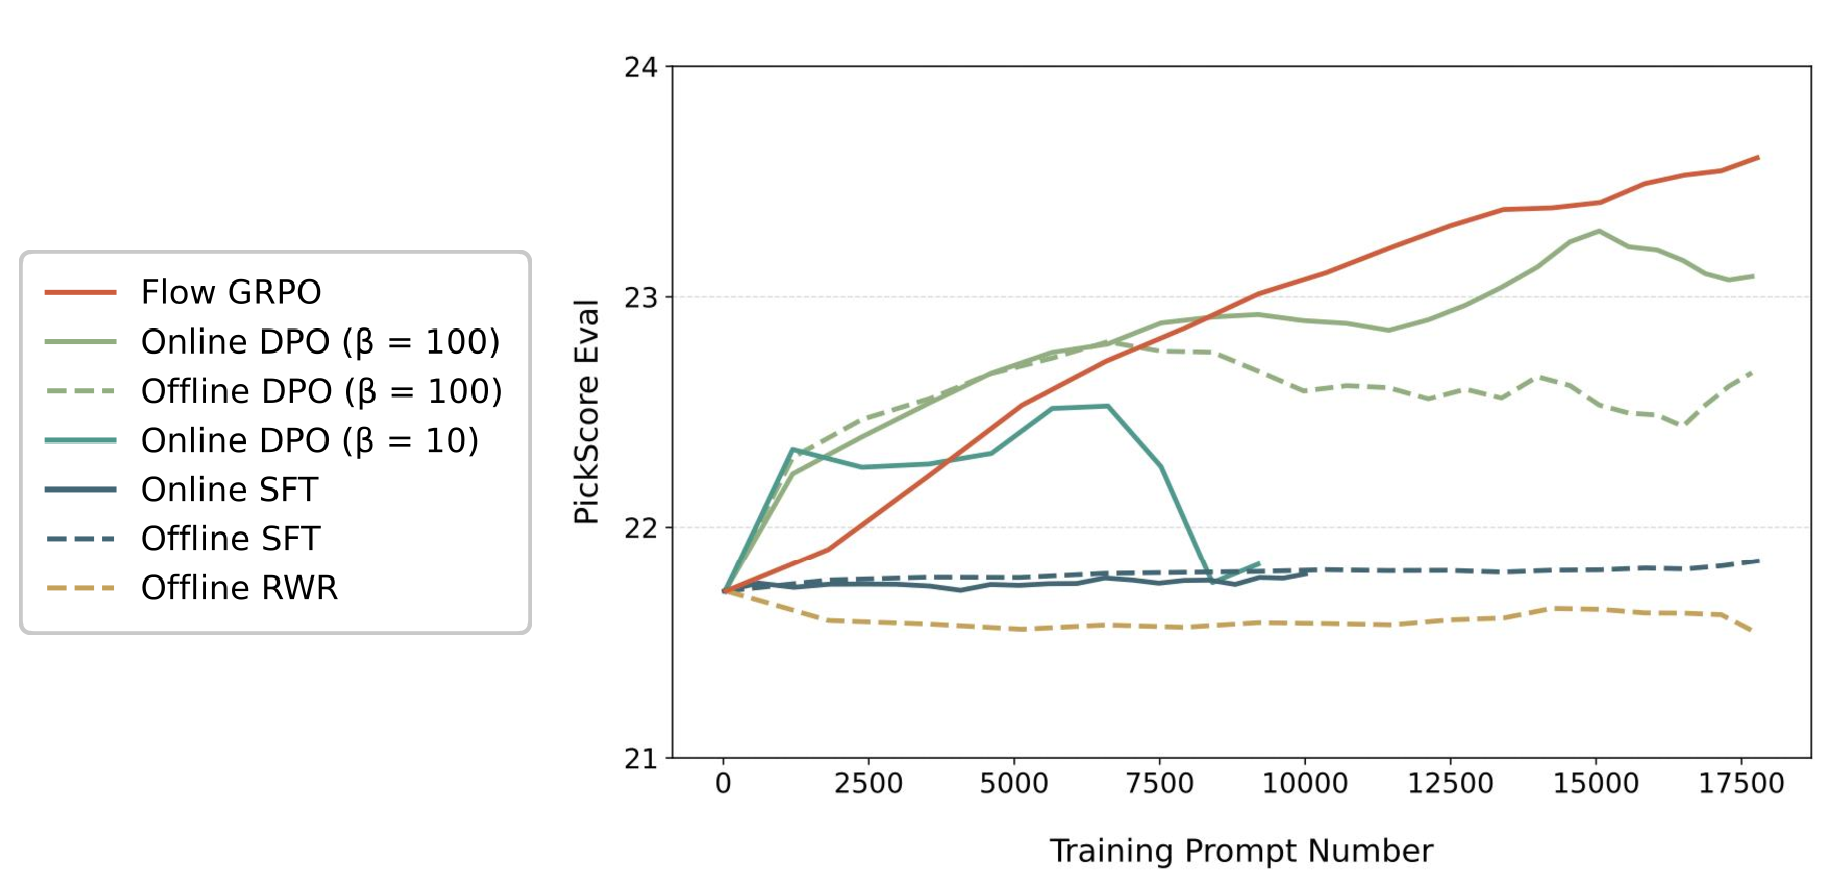
\includegraphics[width=0.9\linewidth]{src/experiments/compare_curve.pdf}
  \end{minipage}
  \begin{minipage}[t]{\textwidth}
    \centering
    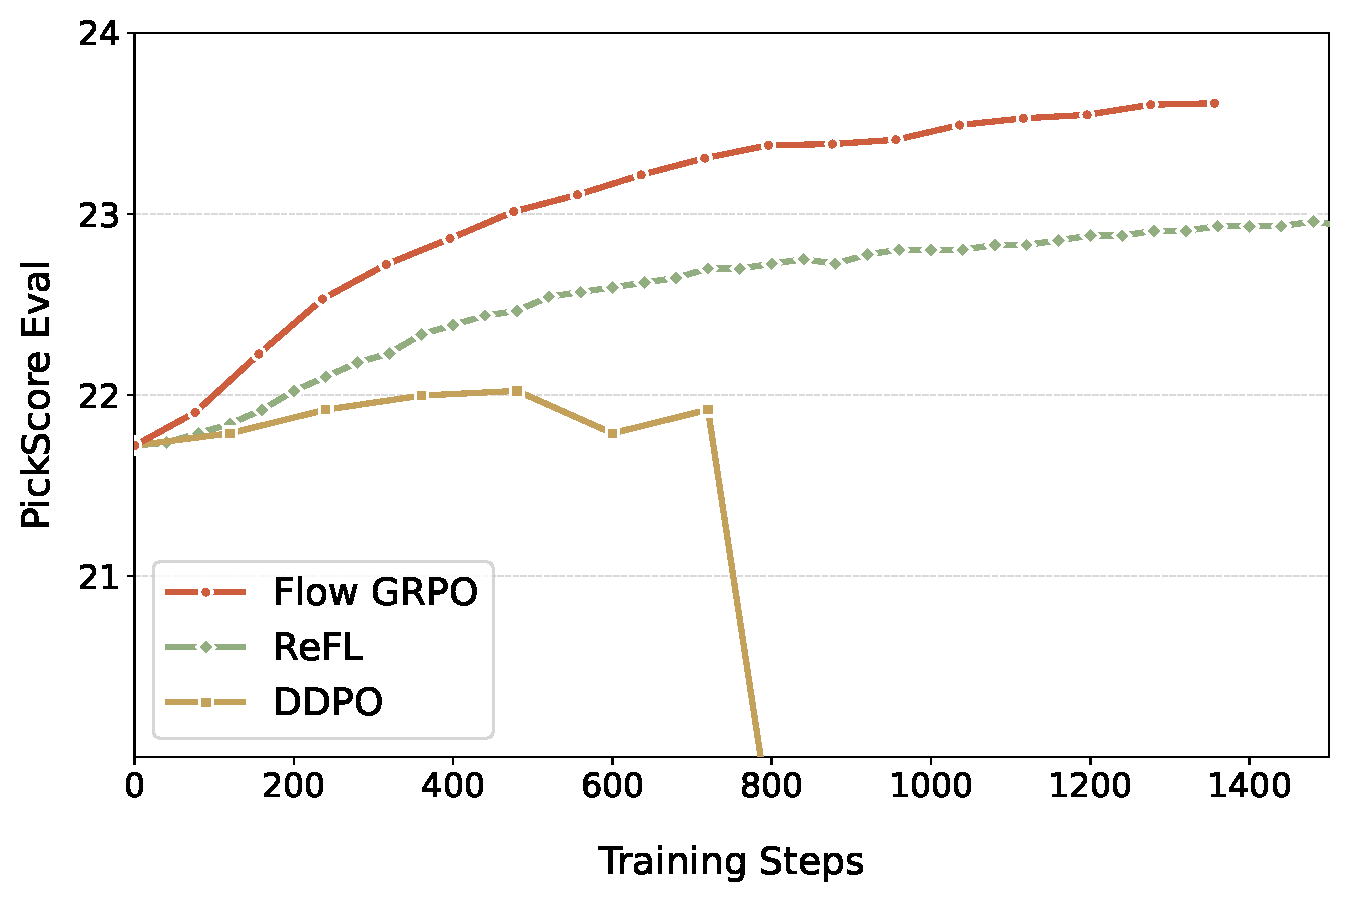
\includegraphics[width=0.6\linewidth]{src/experiments/camera_ready_add/camera_ready_refl.pdf}
  \end{minipage}
    \caption{Comparison of Flow-GRPO and Other Alignment Methods on the Human Preference Alignment task. Since methods like DPO use different tuned batch sizes from Flow-GRPO, we use the number of training prompts on the x-axis for a fair comparison across these methods.
}
  \label{app:fig:compare_curva}
\end{figure}

% \begin{figure}[htbp]
% \centering
% 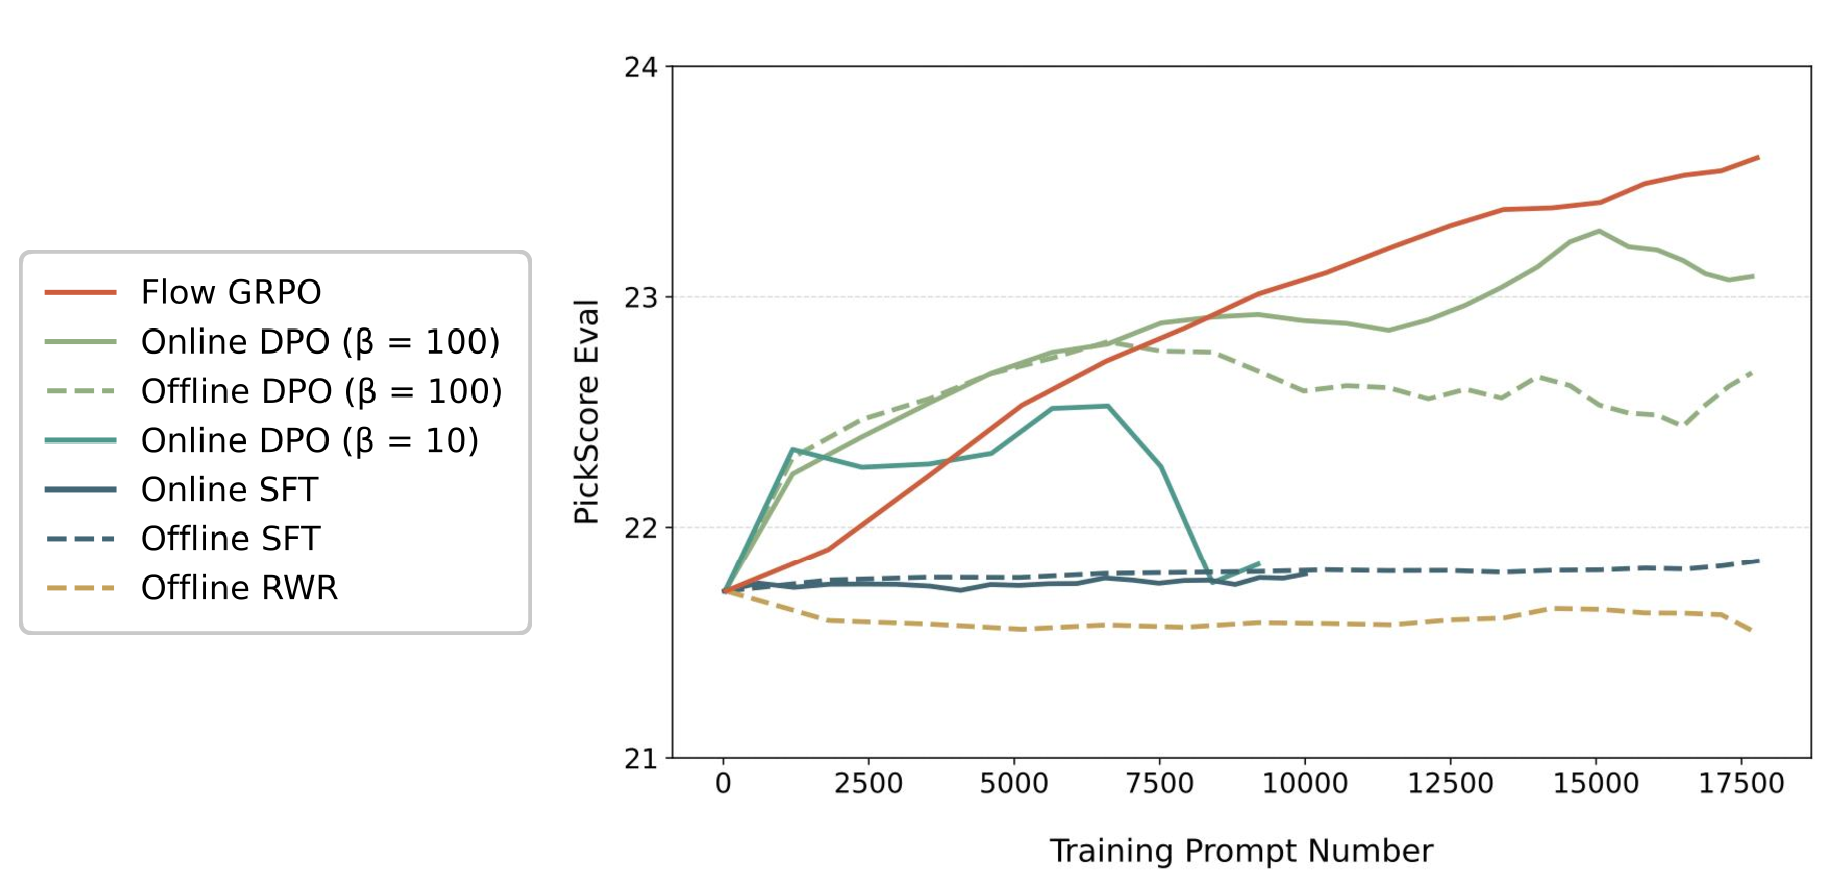
\includegraphics[width=0.9\textwidth]{src/experiments/compare_curve.pdf}
% \caption{Comparison of Flow-GRPO and Other Alignment Methods on the Human Preference Alignment task.
% }
% \label{app:fig:compare_curva}
% \end{figure}

\paragraph{DDPO.} 
DDPO~\cite{ddpo} was originally developed for diffusion-based backbones, so we adapted it to flow-matching models via our ODE-to-SDE conversion. Using SD3.5-M as the base model and PickScore as the reward signal, we track the evaluation reward throughout the entire training process in Figure~\ref{app:fig:compare_curva}. We find that DDPO’s reward increases more slowly than Flow-GRPO’s and eventually collapses in the later stages, whereas Flow-GRPO trains stably and continues to improve consistently over time.

\paragraph{ReFL.}
ReFL~\cite{xu2024imagereward} directly fine-tunes diffusion models by viewing reward model scores as human preference losses and back-propagating gradients to a randomly-picked late timestep $t$.
Following ImageReward~\cite{xu2024imagereward}, we back-propagate gradients to a randomly chosen late timestep $t \in [30, 40]$ during denoising. Figure~\ref{app:fig:compare_curva} shows that GRPO surpasses ReFL when the reward is differentiable, indicating that GRPO maintains strong performance in settings where ReFL applies. More importantly, GRPO does not require differentiable rewards, enabling direct use of state-of-the-art Vision-Language Models (VLMs) as reward providers. This offers two key advantages:

\begin{itemize}[leftmargin=10pt]
\item \textbf{Sophisticated, General-Purpose Rewards:} VLMs can conduct human-like evaluations through a structured reasoning process. Given a prompt, a VLM can decompose it into key criteria, reason step by step to verify each aspect in the generated image, and then provide a comprehensive overall score. This enables a single, unified reward model to handle diverse tasks, from text-to-image generation to complex instruction-based image editing.

\item \textbf{Future-Proof and Cost-Free Upgrades:} The field of VLMs is advancing at a breathtaking pace. By using a VLM as the reward source, our framework automatically benefits from these improvements. As VLMs become more capable, the reward model becomes stronger without any additional training data or computational cost.
\end{itemize}


\paragraph{ORW.}
ORW~\cite{fan2025online} is an online reward-weighted regression method that guides the model to prioritize high-reward regions. Unlike KL regularization, it employs Wasserstein-2 regularization to prevent policy collapse and maintain diversity.
To ensure a fair comparison, we adopt the same experimental setup as in our Human Preference Alignment task.
For ORW, we set $\beta = 0.5$ and $\alpha = 1$ (lower values led to unstable training). The $\text{steps\_per\_epoch}$ parameter, which controls how frequently the data-collecting policy is updated, was chosen from ${20, 40, 100, 400}$ based on best performance.
Table~\ref{tab:sd35_flowgrpo_orw} reports reward scores on the test set across training steps.
Following ORW’s Table 1, we randomly sampled 50 DrawBench prompts and generated 64 images per prompt to compute CLIP and Diversity scores.
As shown in Table~\ref{tab:clip_diversity_scores}, Flow-GRPO outperforms ORW on both metrics.

\begin{table}[h]
\centering
\small
\caption{Reward scores on the test set over training steps.}
\begin{tabular}{lccccc}
\toprule
\textbf{Method} & \textbf{Step 0} & \textbf{Step 240} & \textbf{Step 480} & \textbf{Step 720} & \textbf{Step 960} \\
\midrule
SD3.5-M + ORW & 28.79 & 29.05 & 29.15 & 27.58 & 23.05 \\
\textbf{SD3.5-M + Flow-GRPO} & 28.79 & \textbf{29.10} & \textbf{29.17} & \textbf{29.51} & \textbf{29.89} \\
\bottomrule
\end{tabular}
\label{tab:sd35_flowgrpo_orw}
\end{table}

\begin{table}[h]
\centering
\small
\setlength{\tabcolsep}{24pt}
\caption{Comparison of CLIP and diversity scores across different fine-tuning methods.}
\begin{tabular}{lcc}
\toprule
\textbf{Method} & \textbf{CLIP Score} $\uparrow$ & \textbf{Diversity Score} $\uparrow$ \\
\midrule
SD3.5-M & 27.99 & 0.96 \\
SD3.5-M + ORW & 28.40 & 0.97 \\
\textbf{SD3.5-M + Flow-GRPO} & \textbf{30.18} & \textbf{1.02} \\
\bottomrule
\end{tabular}
\label{tab:clip_diversity_scores}
\end{table}



\subsection{Effect of Denoising Reduction}\label{app:subsec:noising_reduction}
We show the extended Denoising Reduction ablations of Visual Text Rendering and Human Preference Alignment tasks in Figure~\ref{app:fig:exp2_ablation_step}.
\begin{figure}[htbp]
  \centering
  \begin{minipage}[t]{0.48\textwidth}
    \centering
    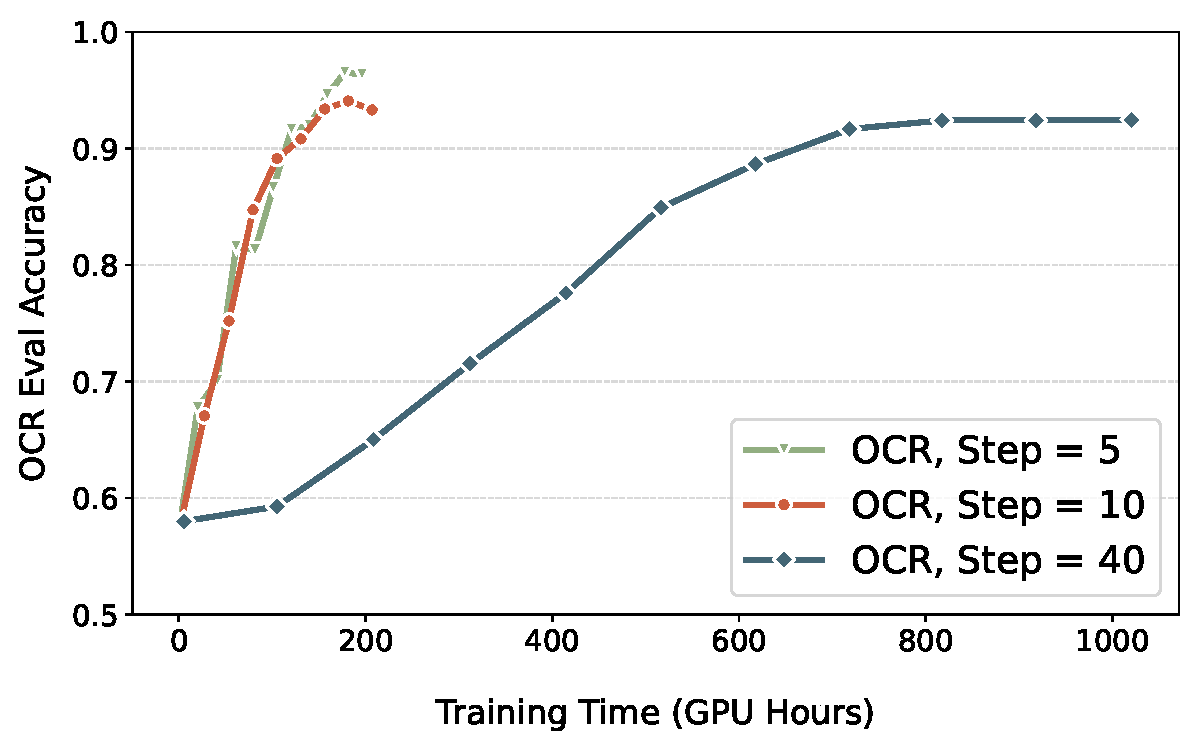
\includegraphics[width=\linewidth]{src/experiments/ablation_step/exp2_ocr_ablation_step.pdf}
    \caption*{\footnotesize (a) Visual Text Rendering}
  \end{minipage}
  \begin{minipage}[t]{0.48\textwidth}
    \centering
    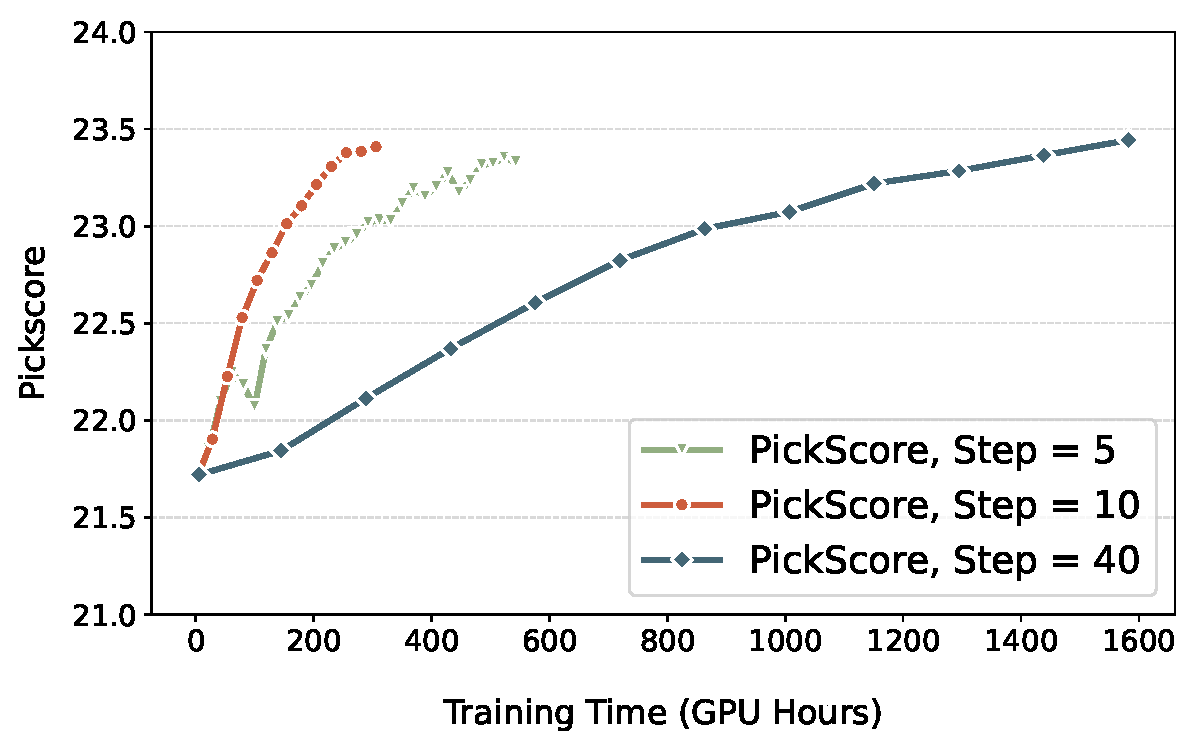
\includegraphics[width=\linewidth]{src/experiments/ablation_step/exp2_pickscore_ablation_step.pdf}
    \vspace{-1.5em}
    \caption*{\footnotesize (b) Human Preference Alignment}
  \end{minipage}
    \caption{Effect of Denoising Reduction}
  \label{app:fig:exp2_ablation_step}
\end{figure}

\subsection{Effect of Initial Noise}\label{app:subsec:initial_noise}
We initialize each rollout with difference random noise to increase exploratory diversity during RL training. We perform an additioanl ablation to confirm this claim. With SD3.5-M as the base model and PickScore as the reward, we compare Flow-GRPO with different initial noise against Flow-GRPO with the same initial noise. Figure~\ref{app:fig:effect_initial_noise} shows the variant with different noise consistently achieved high rewards during the training process. 

\newpage

% \begin{figure}[htbp]
% \centering
% 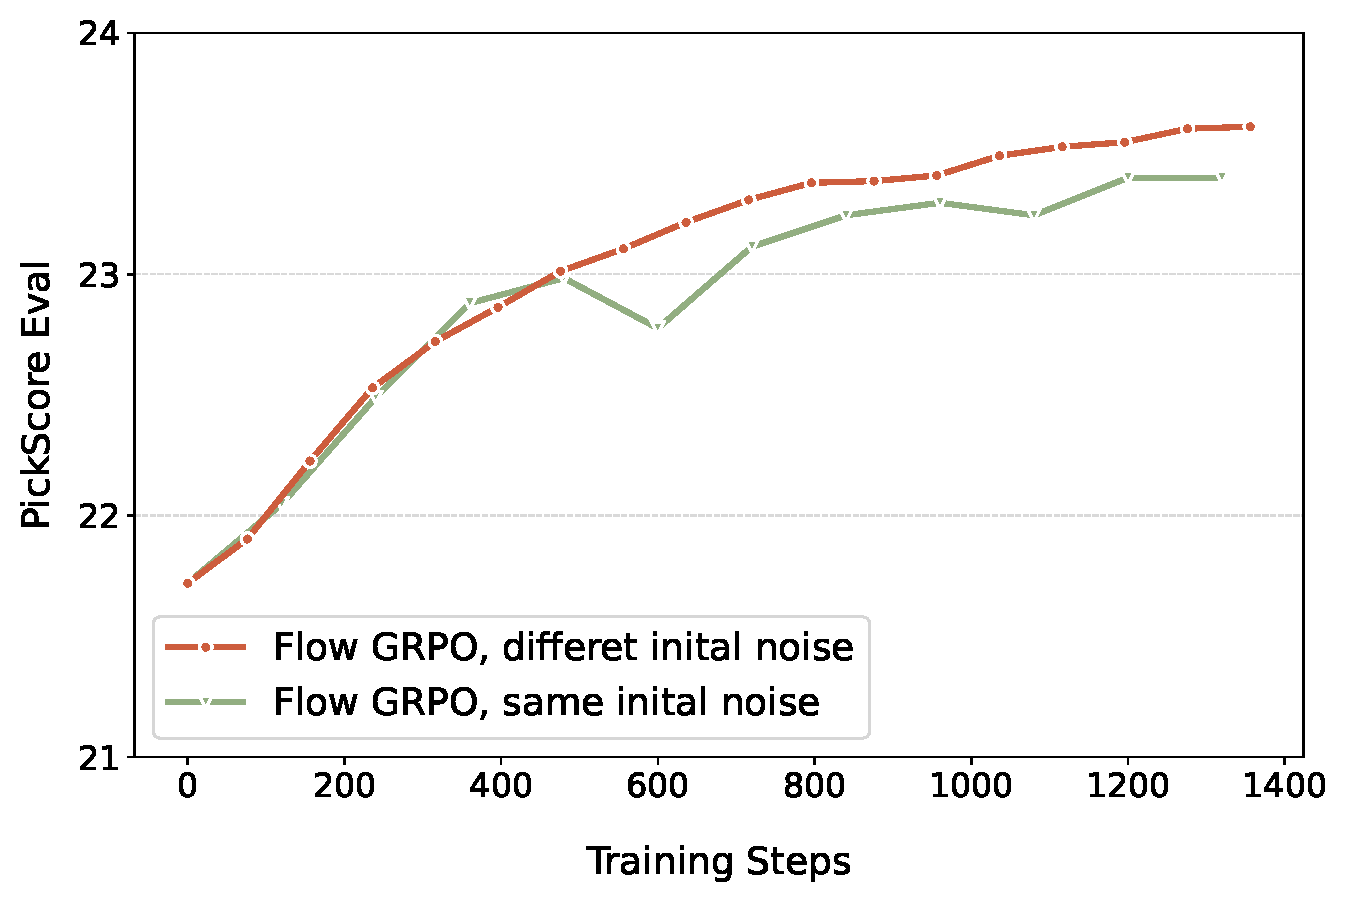
\includegraphics[width=0.6\textwidth]{src/experiments/camera_ready_add/camera_ready_noise.pdf}
% \caption{Effect of Initial Noise.
% }
% \label{app:fig:effect_initial_noise}
% \end{figure}

\begin{figure}[htbp]
  \centering
  \begin{minipage}[t]{0.48\textwidth}
    \centering
    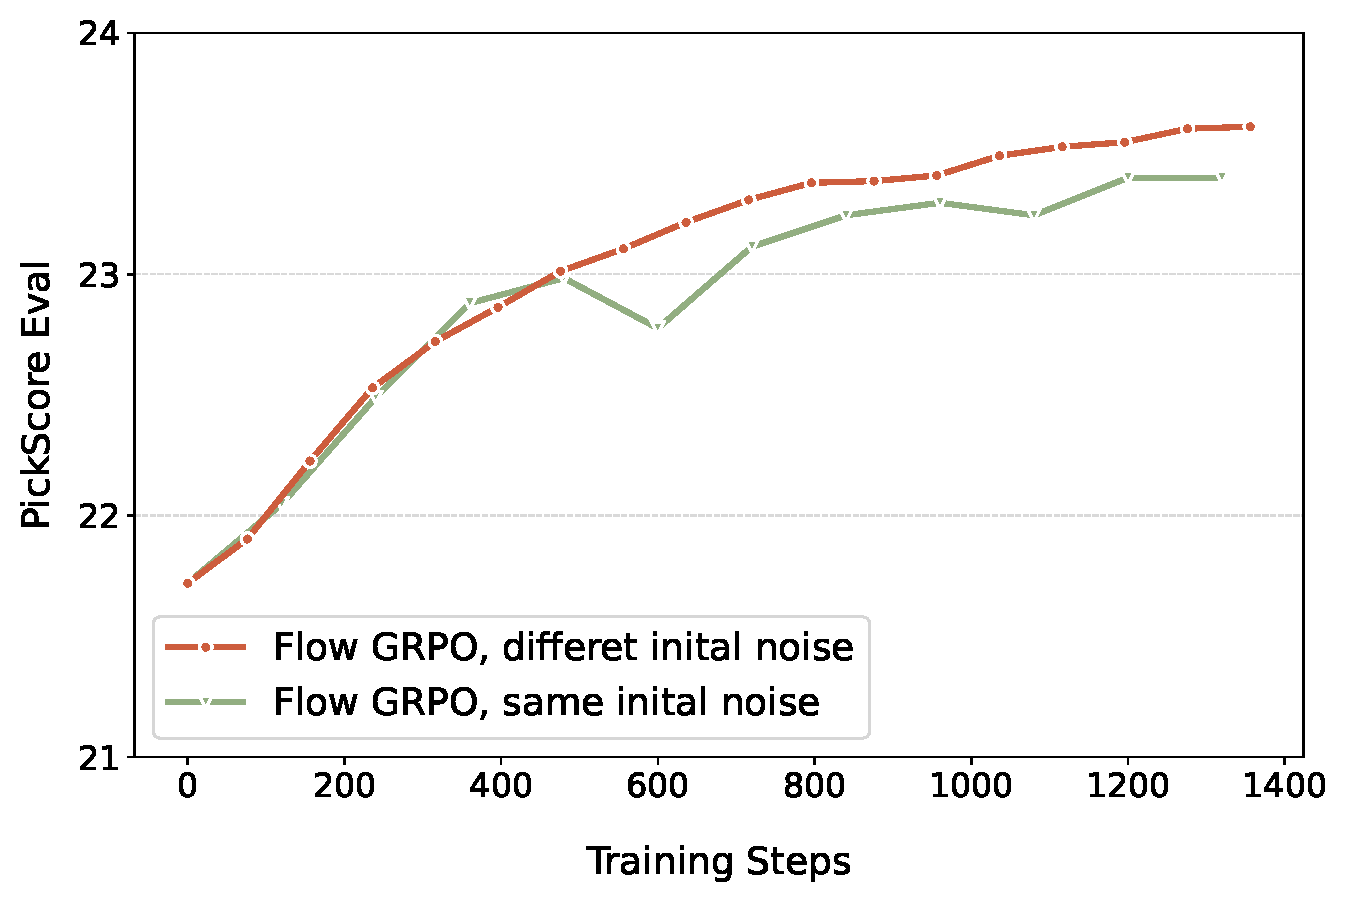
\includegraphics[width=\linewidth]{src/experiments/camera_ready_add/camera_ready_noise.pdf}
    \caption{Effect of Initial Noise}
    \label{app:fig:effect_initial_noise}
  \end{minipage}
  \begin{minipage}[t]{0.48\textwidth}
    \centering
    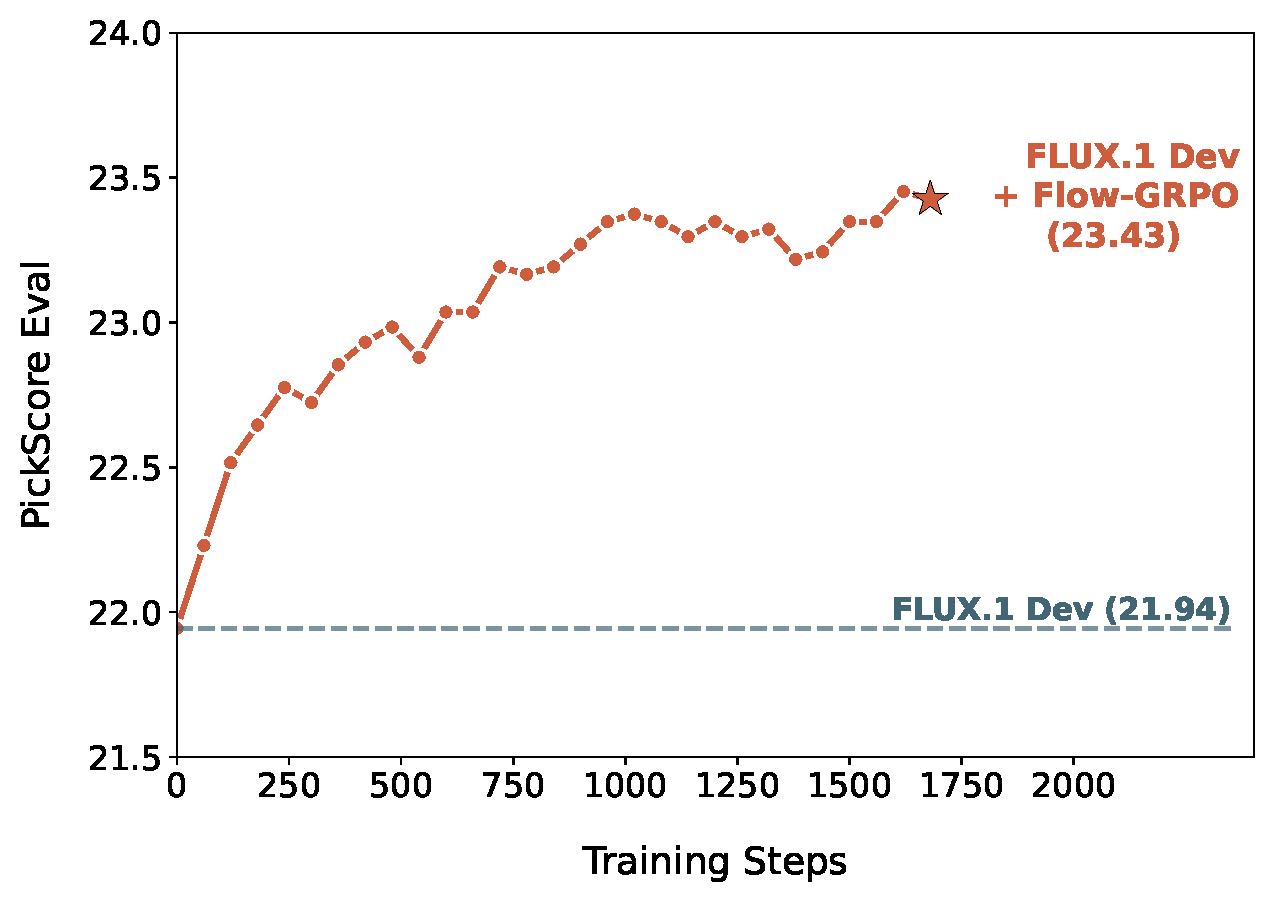
\includegraphics[width=\linewidth]{src/experiments/camera_ready_add/camera_ready_flux.pdf}
    \caption{Additional Results on FLUX.1-Dev}
    \label{app:fig:effect_flux}
  \end{minipage}
\end{figure}


\subsection{Additional Results on FLUX.1-Dev}\label{app:subsec:flux}
We run Flow-GRPO on FLUX.1-Dev~\cite{flux2024} using PickScore as the reward signal. The reward curve rises steadily throughout training without noticeable reward hacking. Figure~\ref{app:fig:effect_flux} shows the reward values over the training process, and Table~\ref{tab:flux_flowgrpo_results} compares FLUX.1-Dev with FLUX.1-Dev + Flow-GRPO on DrawBench.

\begin{table}[h]
\centering
\small
\caption{Comparison of FLUX.1-Dev and Flow-GRPO fine-tuned models.}
\begin{tabular}{lccccc}
\toprule
\textbf{Model} & \textbf{Aesthetic} & \textbf{DeQA} & \textbf{ImageReward} & \textbf{PickScore} & \textbf{UnifiedReward} \\
\midrule
FLUX.1-Dev & 5.71 & 4.31 & 0.85 & 22.62 & 3.65 \\
FLUX.1-Dev + Flow-GRPO & 6.02 & 4.24 & 1.32 & 23.97 & 3.81 \\
\bottomrule
\end{tabular}
\label{tab:flux_flowgrpo_results}
\end{table}

% \vspace{-1em}

% \begin{figure}[h]
% \centering
% 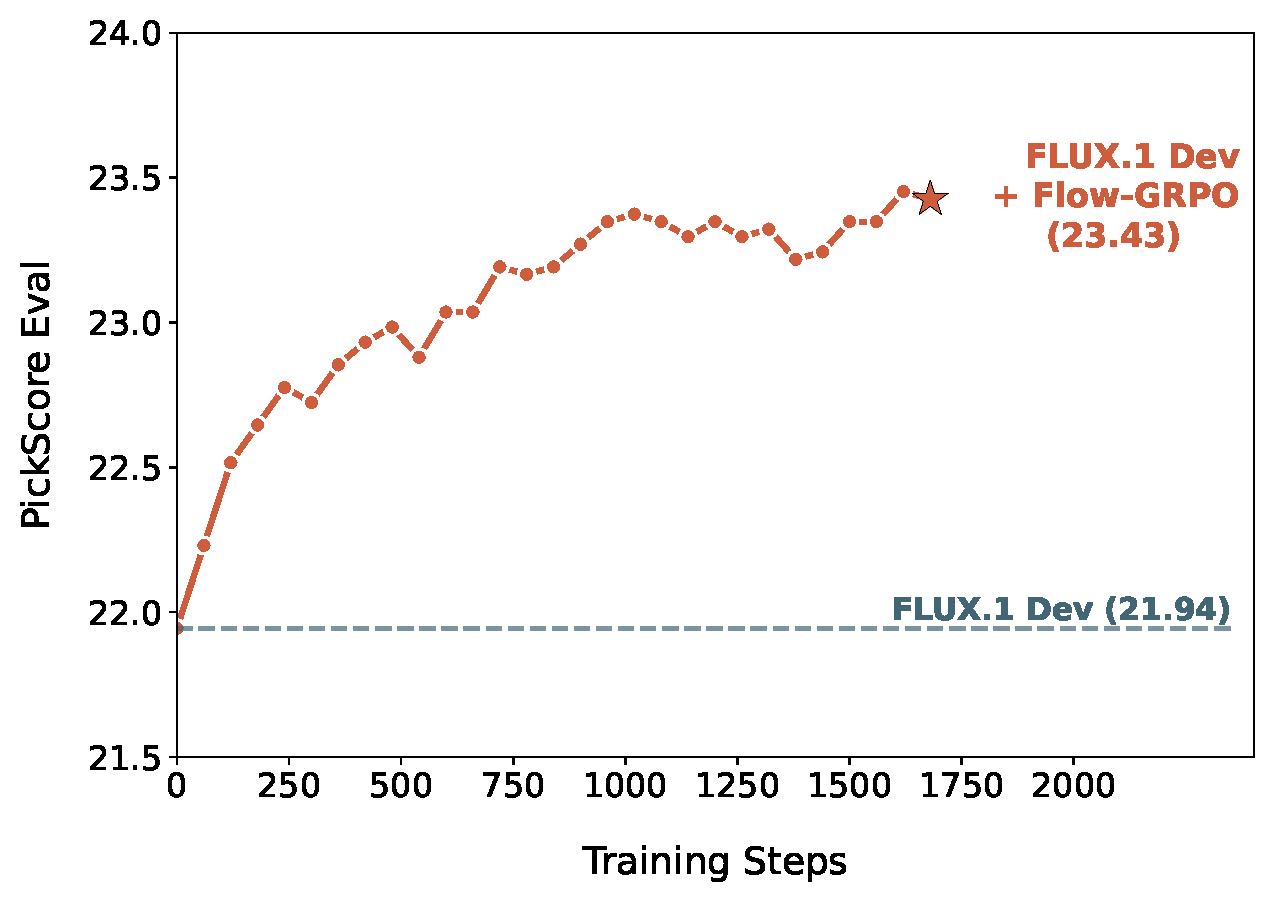
\includegraphics[width=0.6\textwidth]{src/experiments/camera_ready_add/camera_ready_flux.pdf}
% \caption{Additional Results on FLUX.1-Dev
% }
% \label{app:fig:effect_flux}
% \end{figure}

\subsection{Learning Curves with or without KL}\label{app:subsec:training_curve_kl}
Figure~\ref{app:fig:exp3_ablation_kl} shows learning curves for three tasks, with and without KL. These results emphasize that KL regularization is not empirically equivalent to early stopping. Adding appropriate KL can achieve the same high reward as the KL-free version and maintain image quality, though it requires longer training.
\begin{figure}[htbp]
  \centering
  \begin{minipage}[t]{0.48\textwidth}
    \centering
    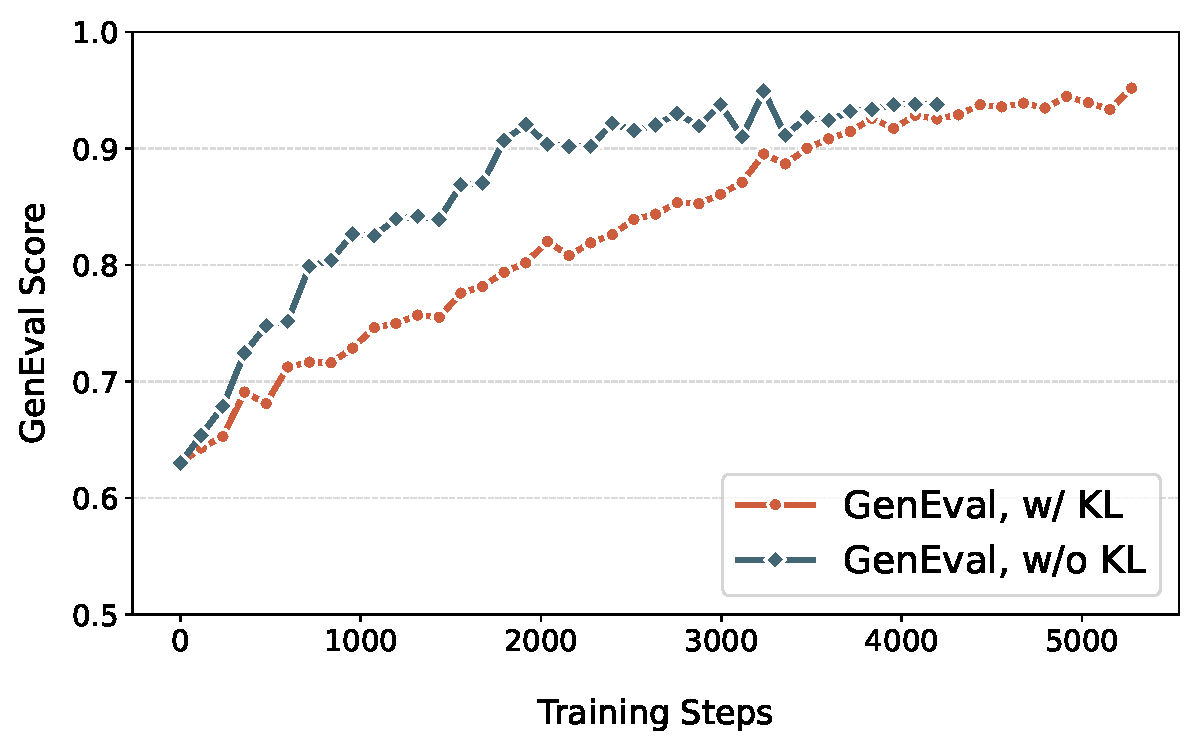
\includegraphics[width=\linewidth]{src/experiments/ablation_kl/exp3_geneval_ablation_kl.pdf}
    \vspace{-1.5em}
    \caption*{\footnotesize (a) Compositional Image Generation}
  \end{minipage}
  \hfill
  \begin{minipage}[t]{0.48\textwidth}
    \centering
    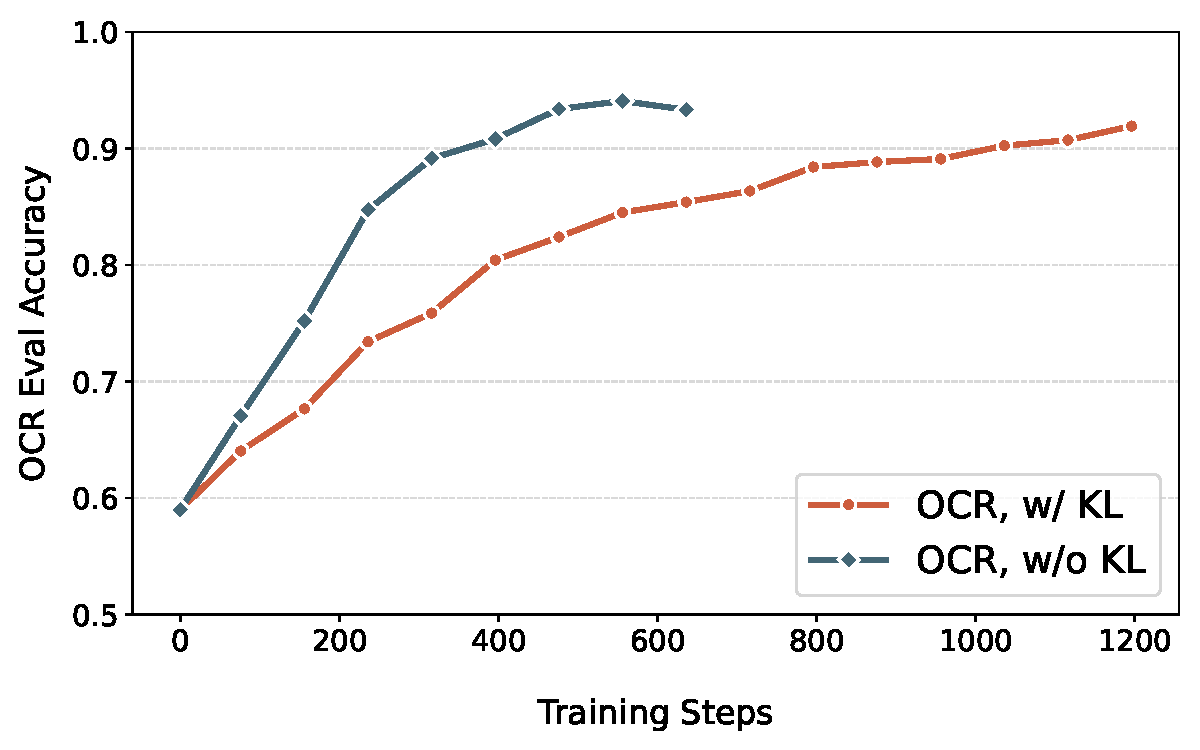
\includegraphics[width=\linewidth]{src/experiments/ablation_kl/exp3_ocr_ablation_kl.pdf}
    \vspace{-1.5em}
    \caption*{\footnotesize (b) Visual Text Rendering}
  \end{minipage}
  \vspace{1.5em}

  \begin{minipage}[t]{0.48\textwidth}
    \centering
    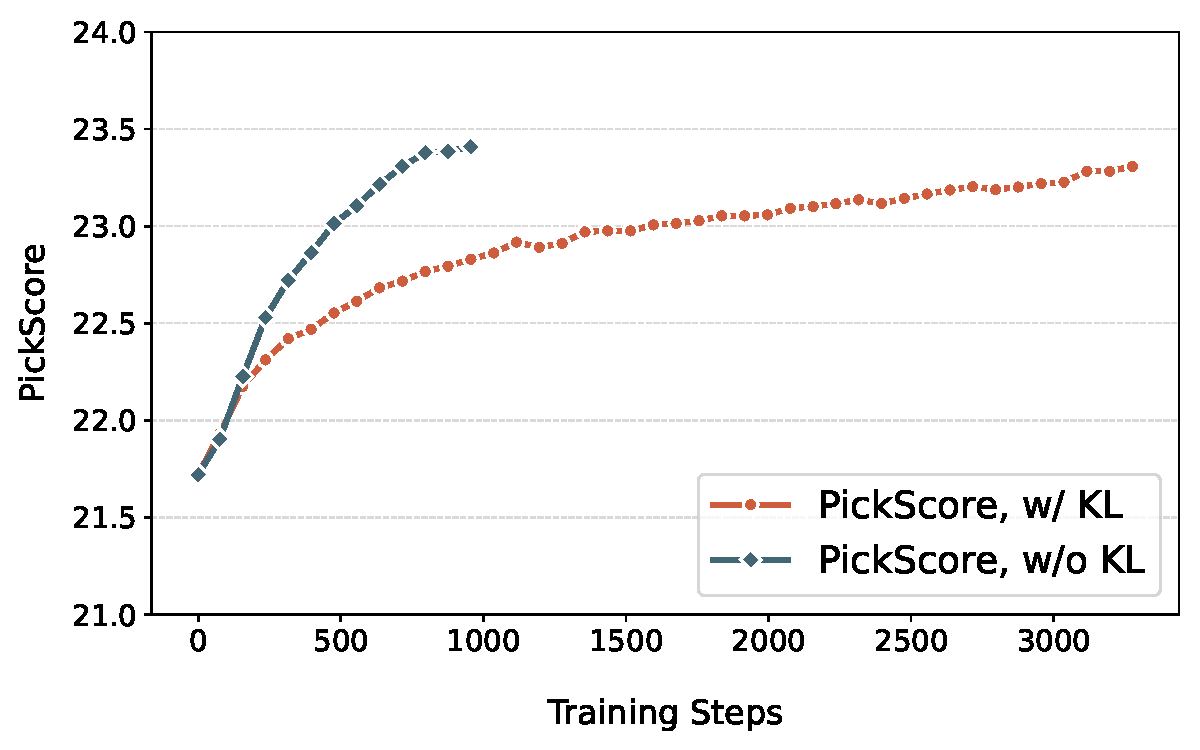
\includegraphics[width=\linewidth]{src/experiments/ablation_kl/exp3_pickscore_ablation_kl.pdf}
    \vspace{-1.5em}
    \caption*{\footnotesize (c) Human Preference Alignment}
  \end{minipage}
  \caption{Learning Curves with and without KL. KL penalty slows early training yet effectively suppresses reward hacking.}
  \label{app:fig:exp3_ablation_kl}
\end{figure}



\subsection{Additional Qualitative Results}\label{app:subsec:qualitative_results}
Figures~\ref{app:fig:add_qualitative_result_geneval}, \ref{app:fig:add_qualitative_result_ocr} \& \ref{app:fig:add_qualitative_result_pickscore} qualitatively compare SD3.5-M with its Flow-GRPO enhanced versions (with and without KL regularization) using GenEval, OCR and PickScore rewards, respectively. Flow-GRPO with KL regularization improves the target capability while maintaining image quality and minimizing reward-hacking. Conversely, removing the KL constraint significantly degrades image quality and diversity.

\begin{figure}[htbp]
\centering
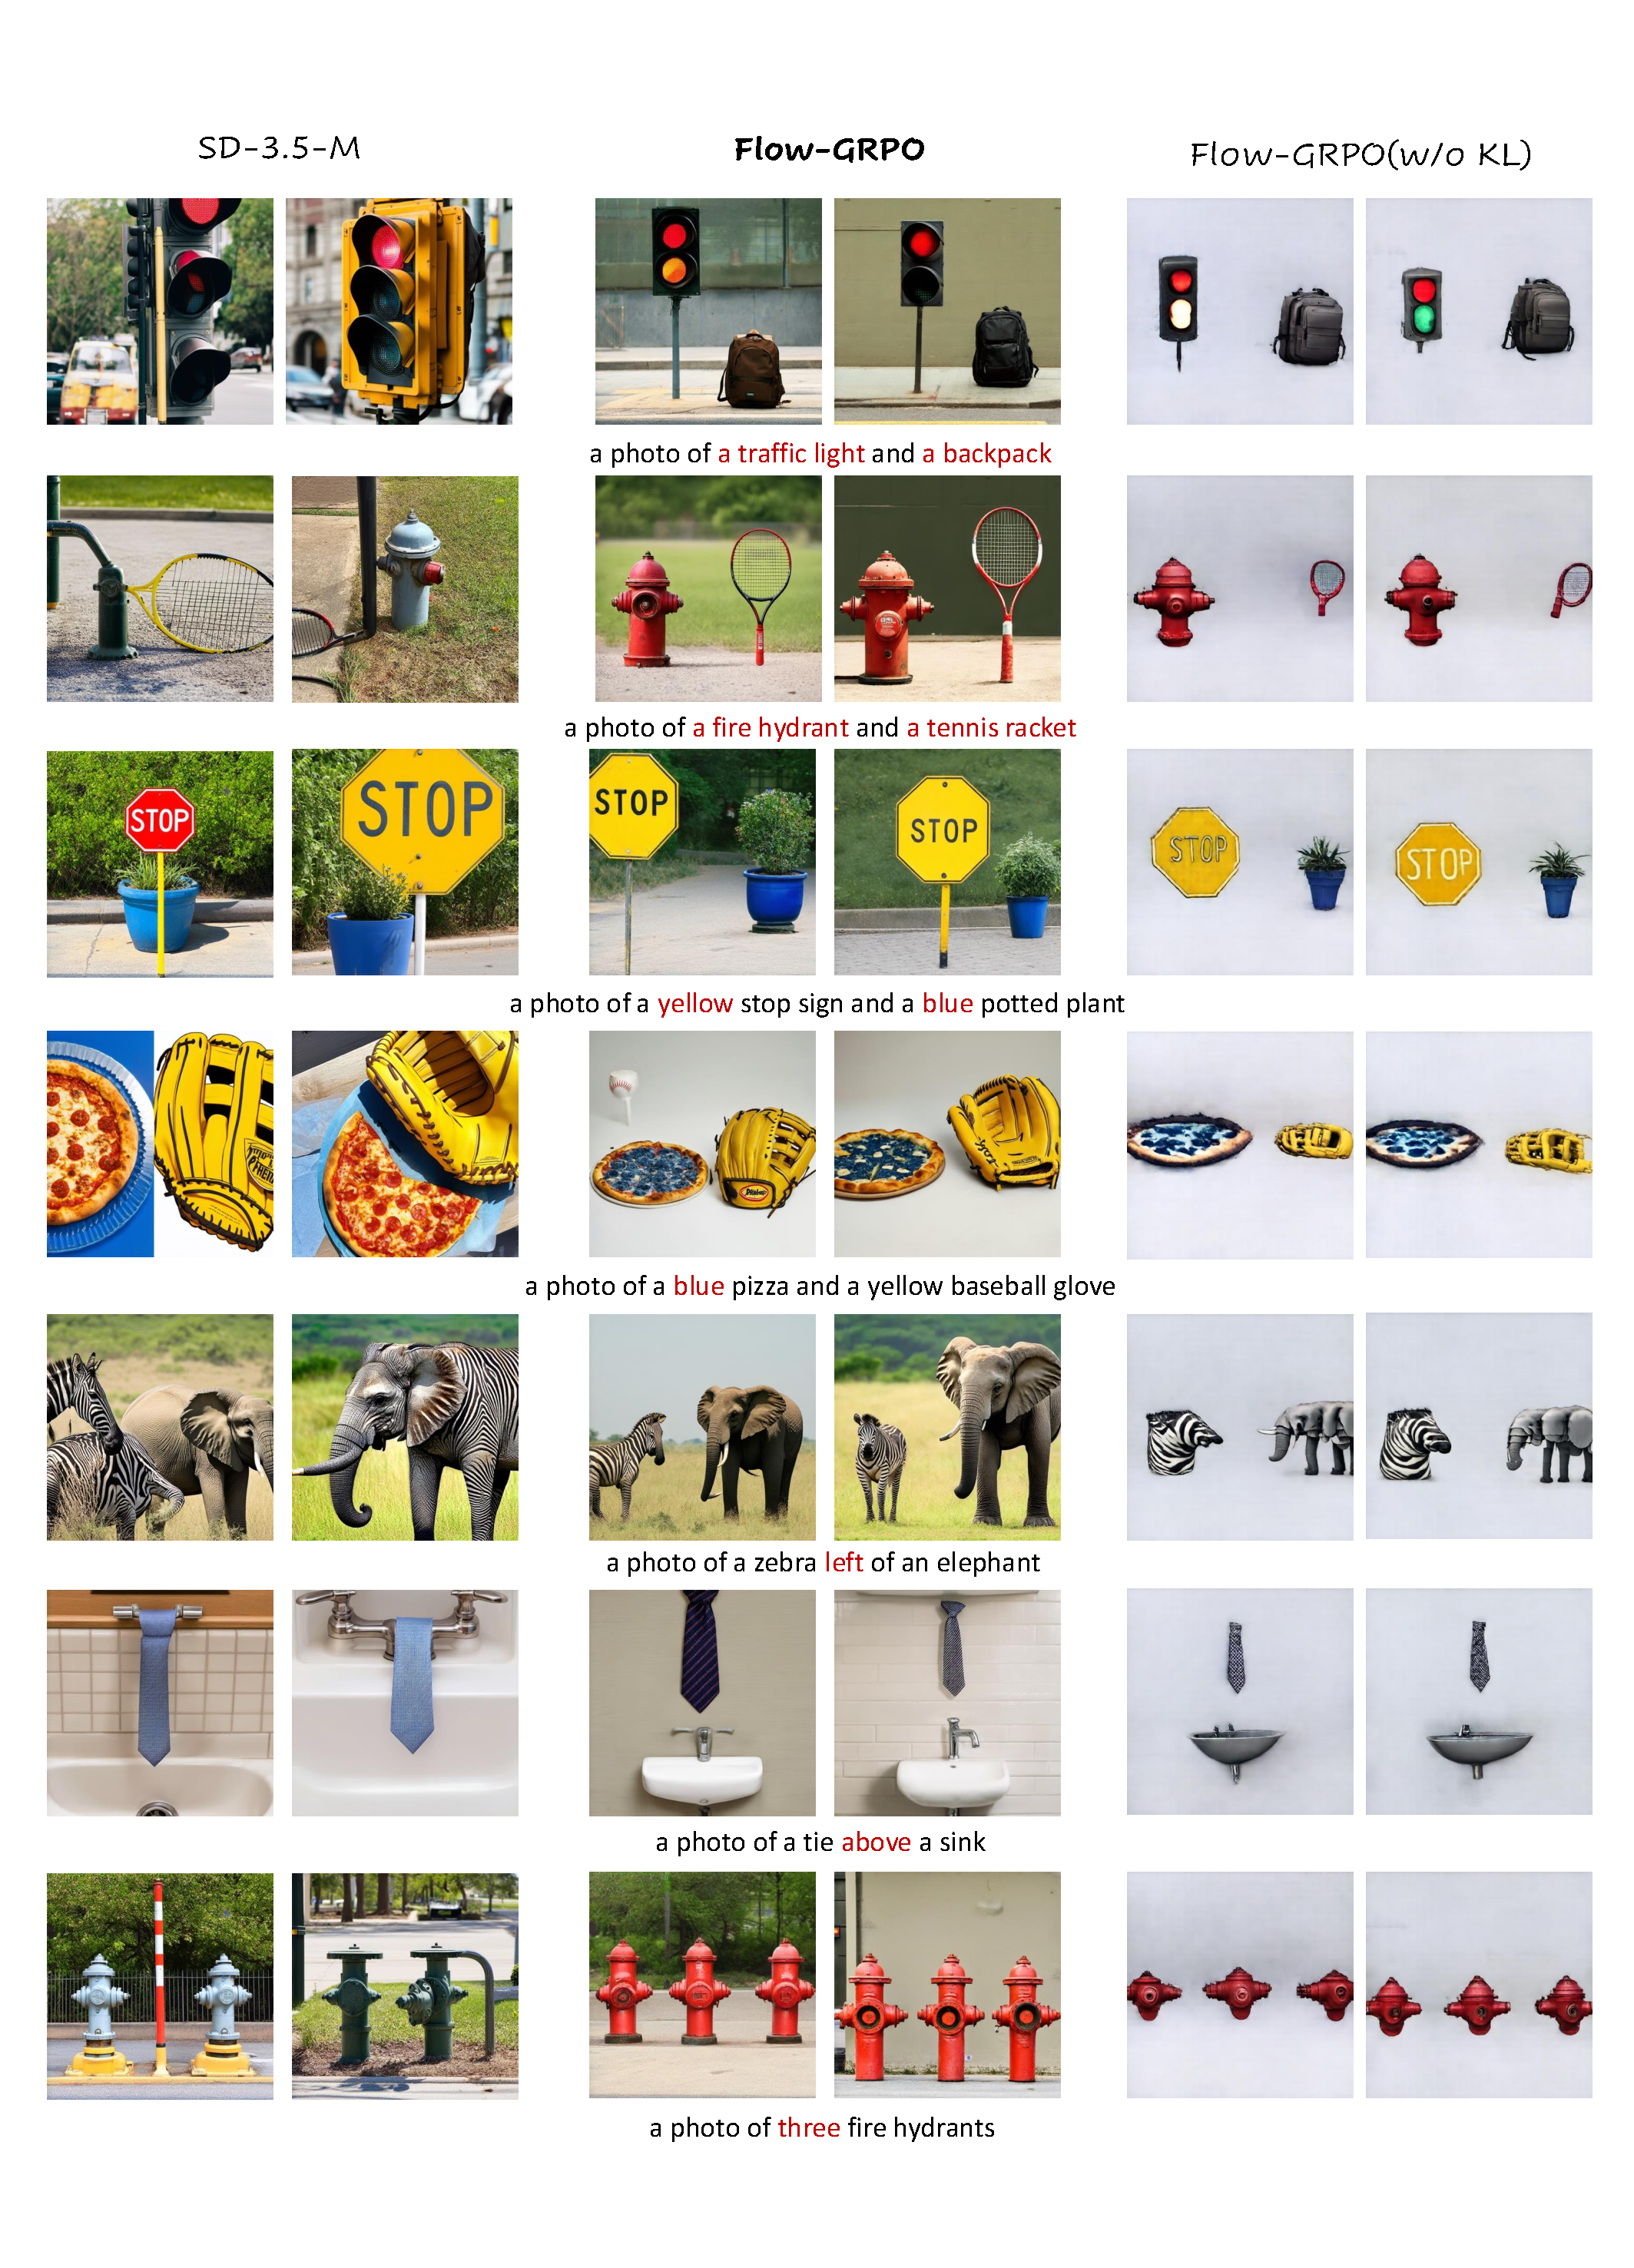
\includegraphics[width=\textwidth]{src/experiments/more_results_geneval.pdf}
\caption{Additional Qualitative comparison between the SD3.5-M and SD3.5-M + Flow-GRPO trained with \textbf{GenEval} reward.
}
\label{app:fig:add_qualitative_result_geneval}
\end{figure}


\begin{figure}[htbp]
\centering
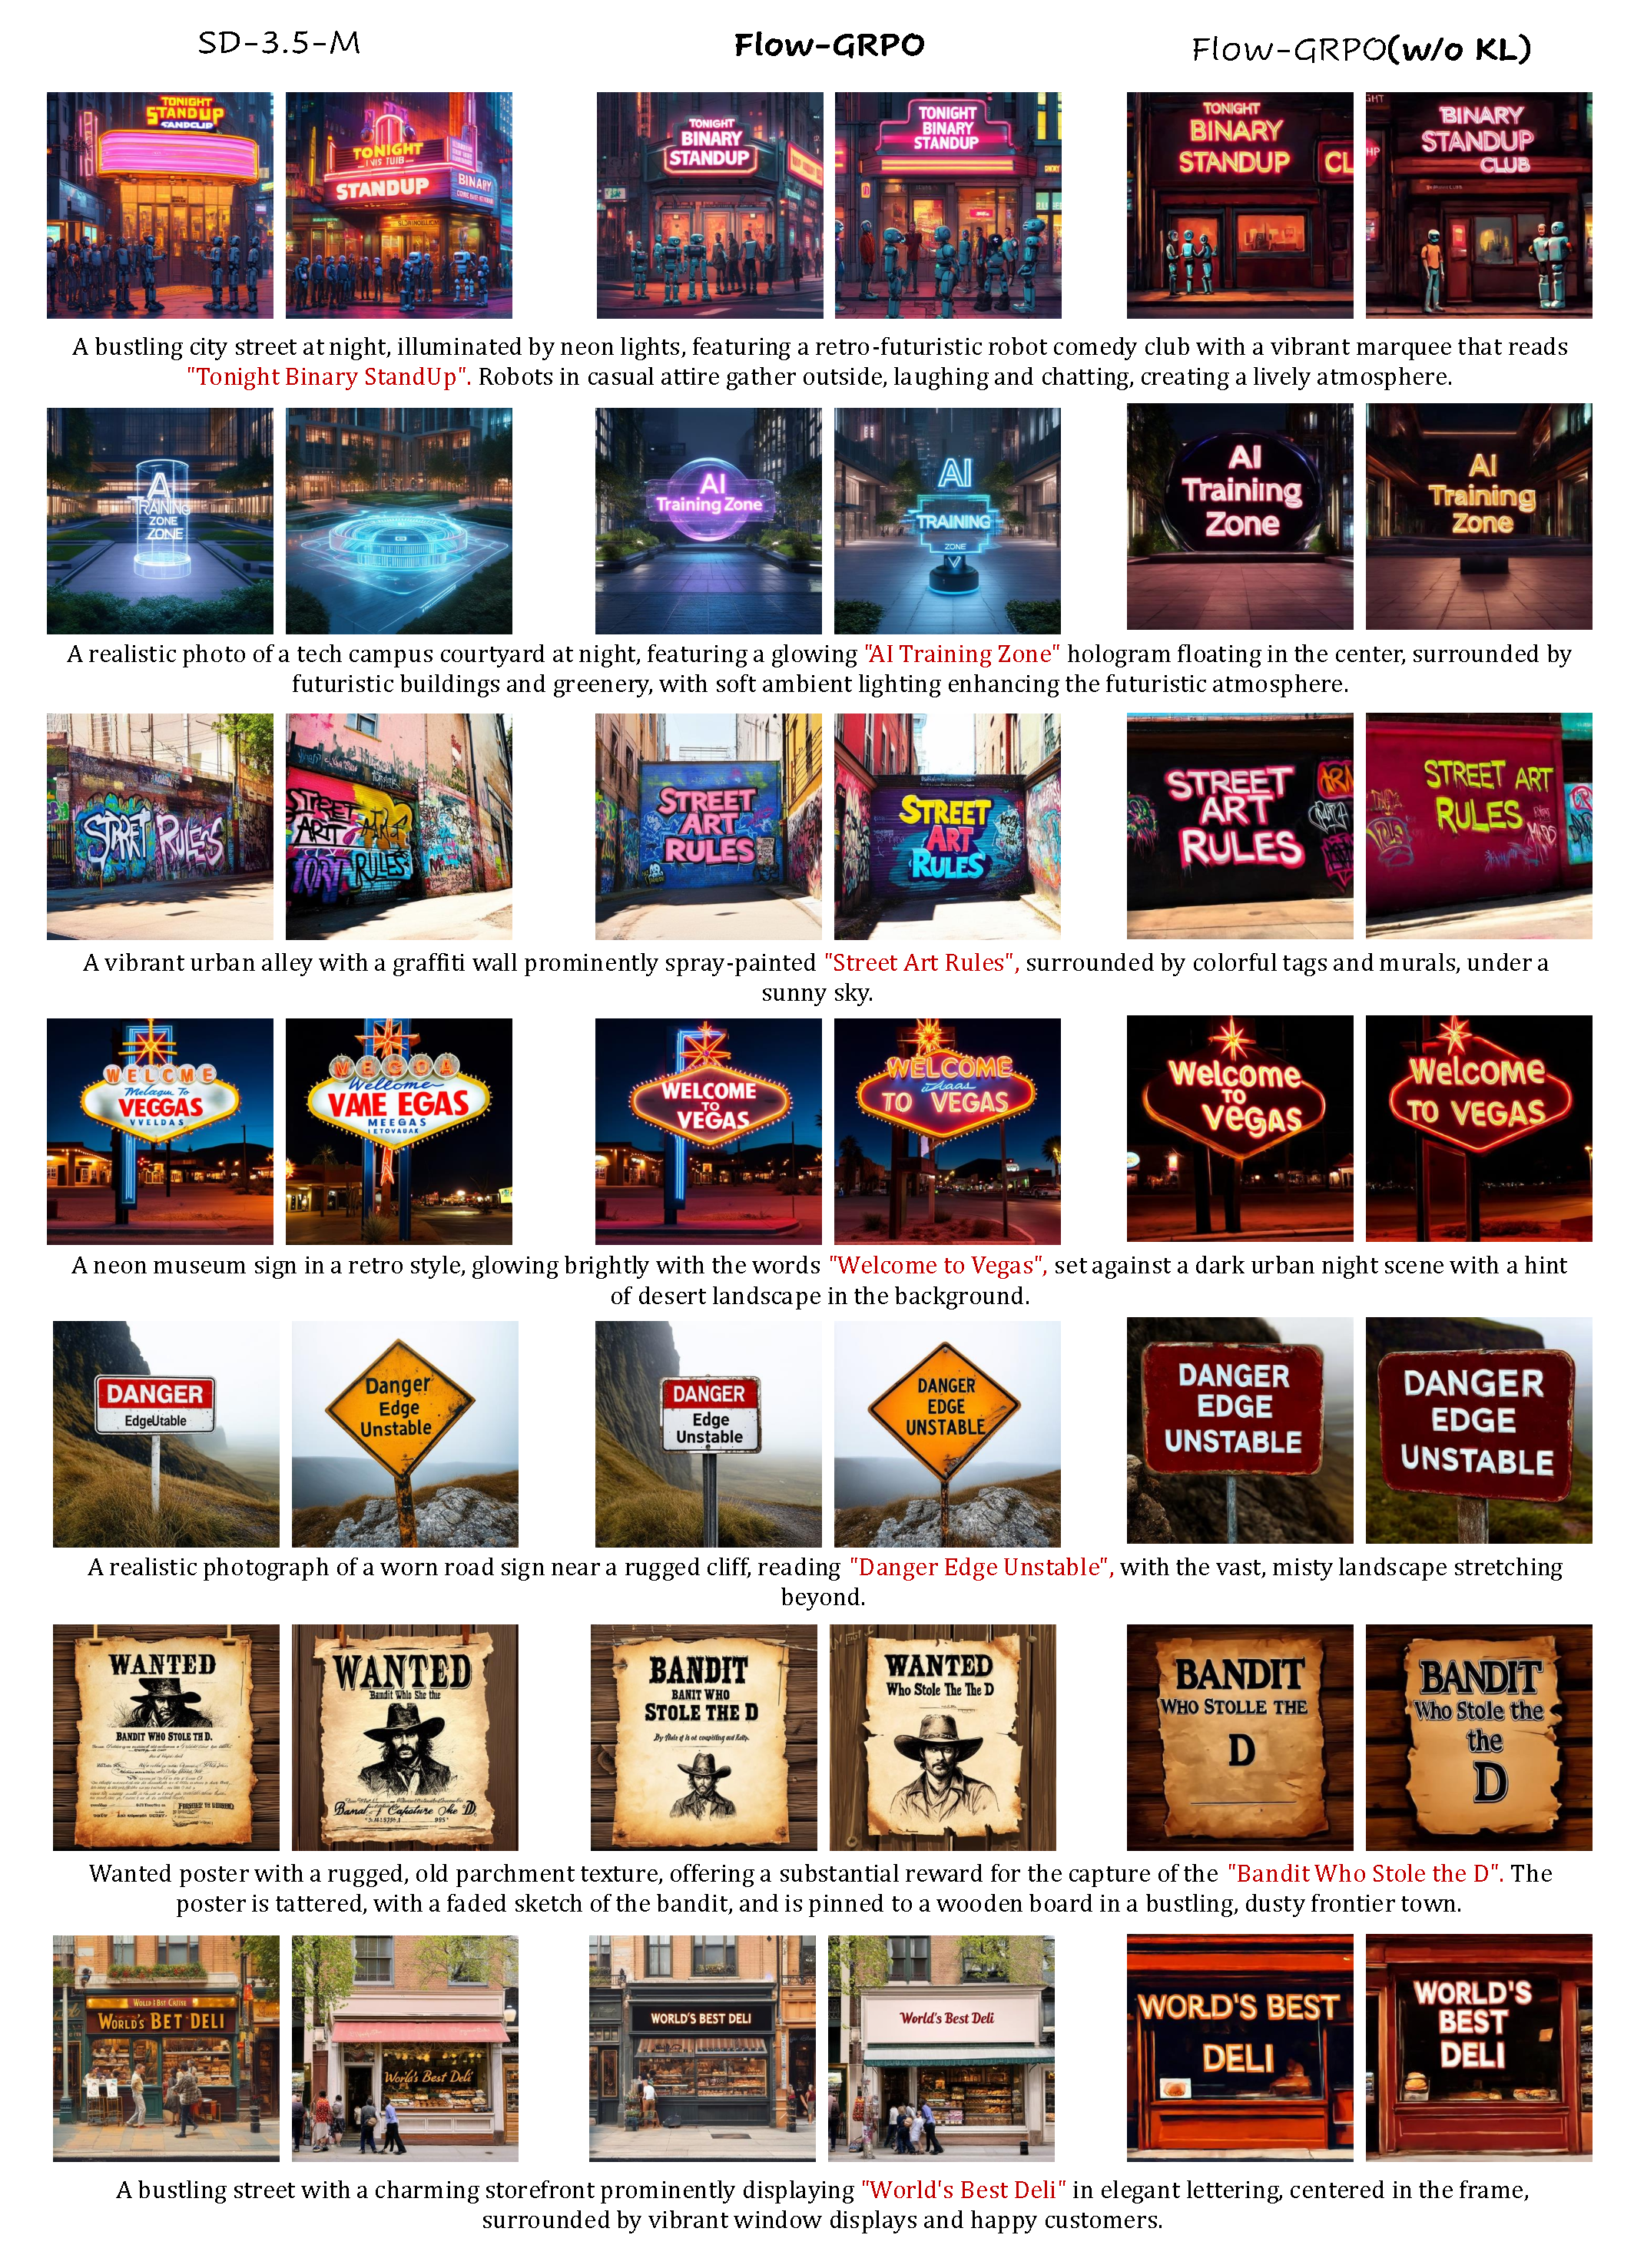
\includegraphics[width=\textwidth]{src/experiments/more_results_ocr.pdf}
\caption{Additional Qualitative comparison between the SD3.5-M and SD3.5-M + Flow-GRPO trained with \textbf{OCR} reward.
}
\label{app:fig:add_qualitative_result_ocr}
\end{figure}

\begin{figure}[htbp]
\centering
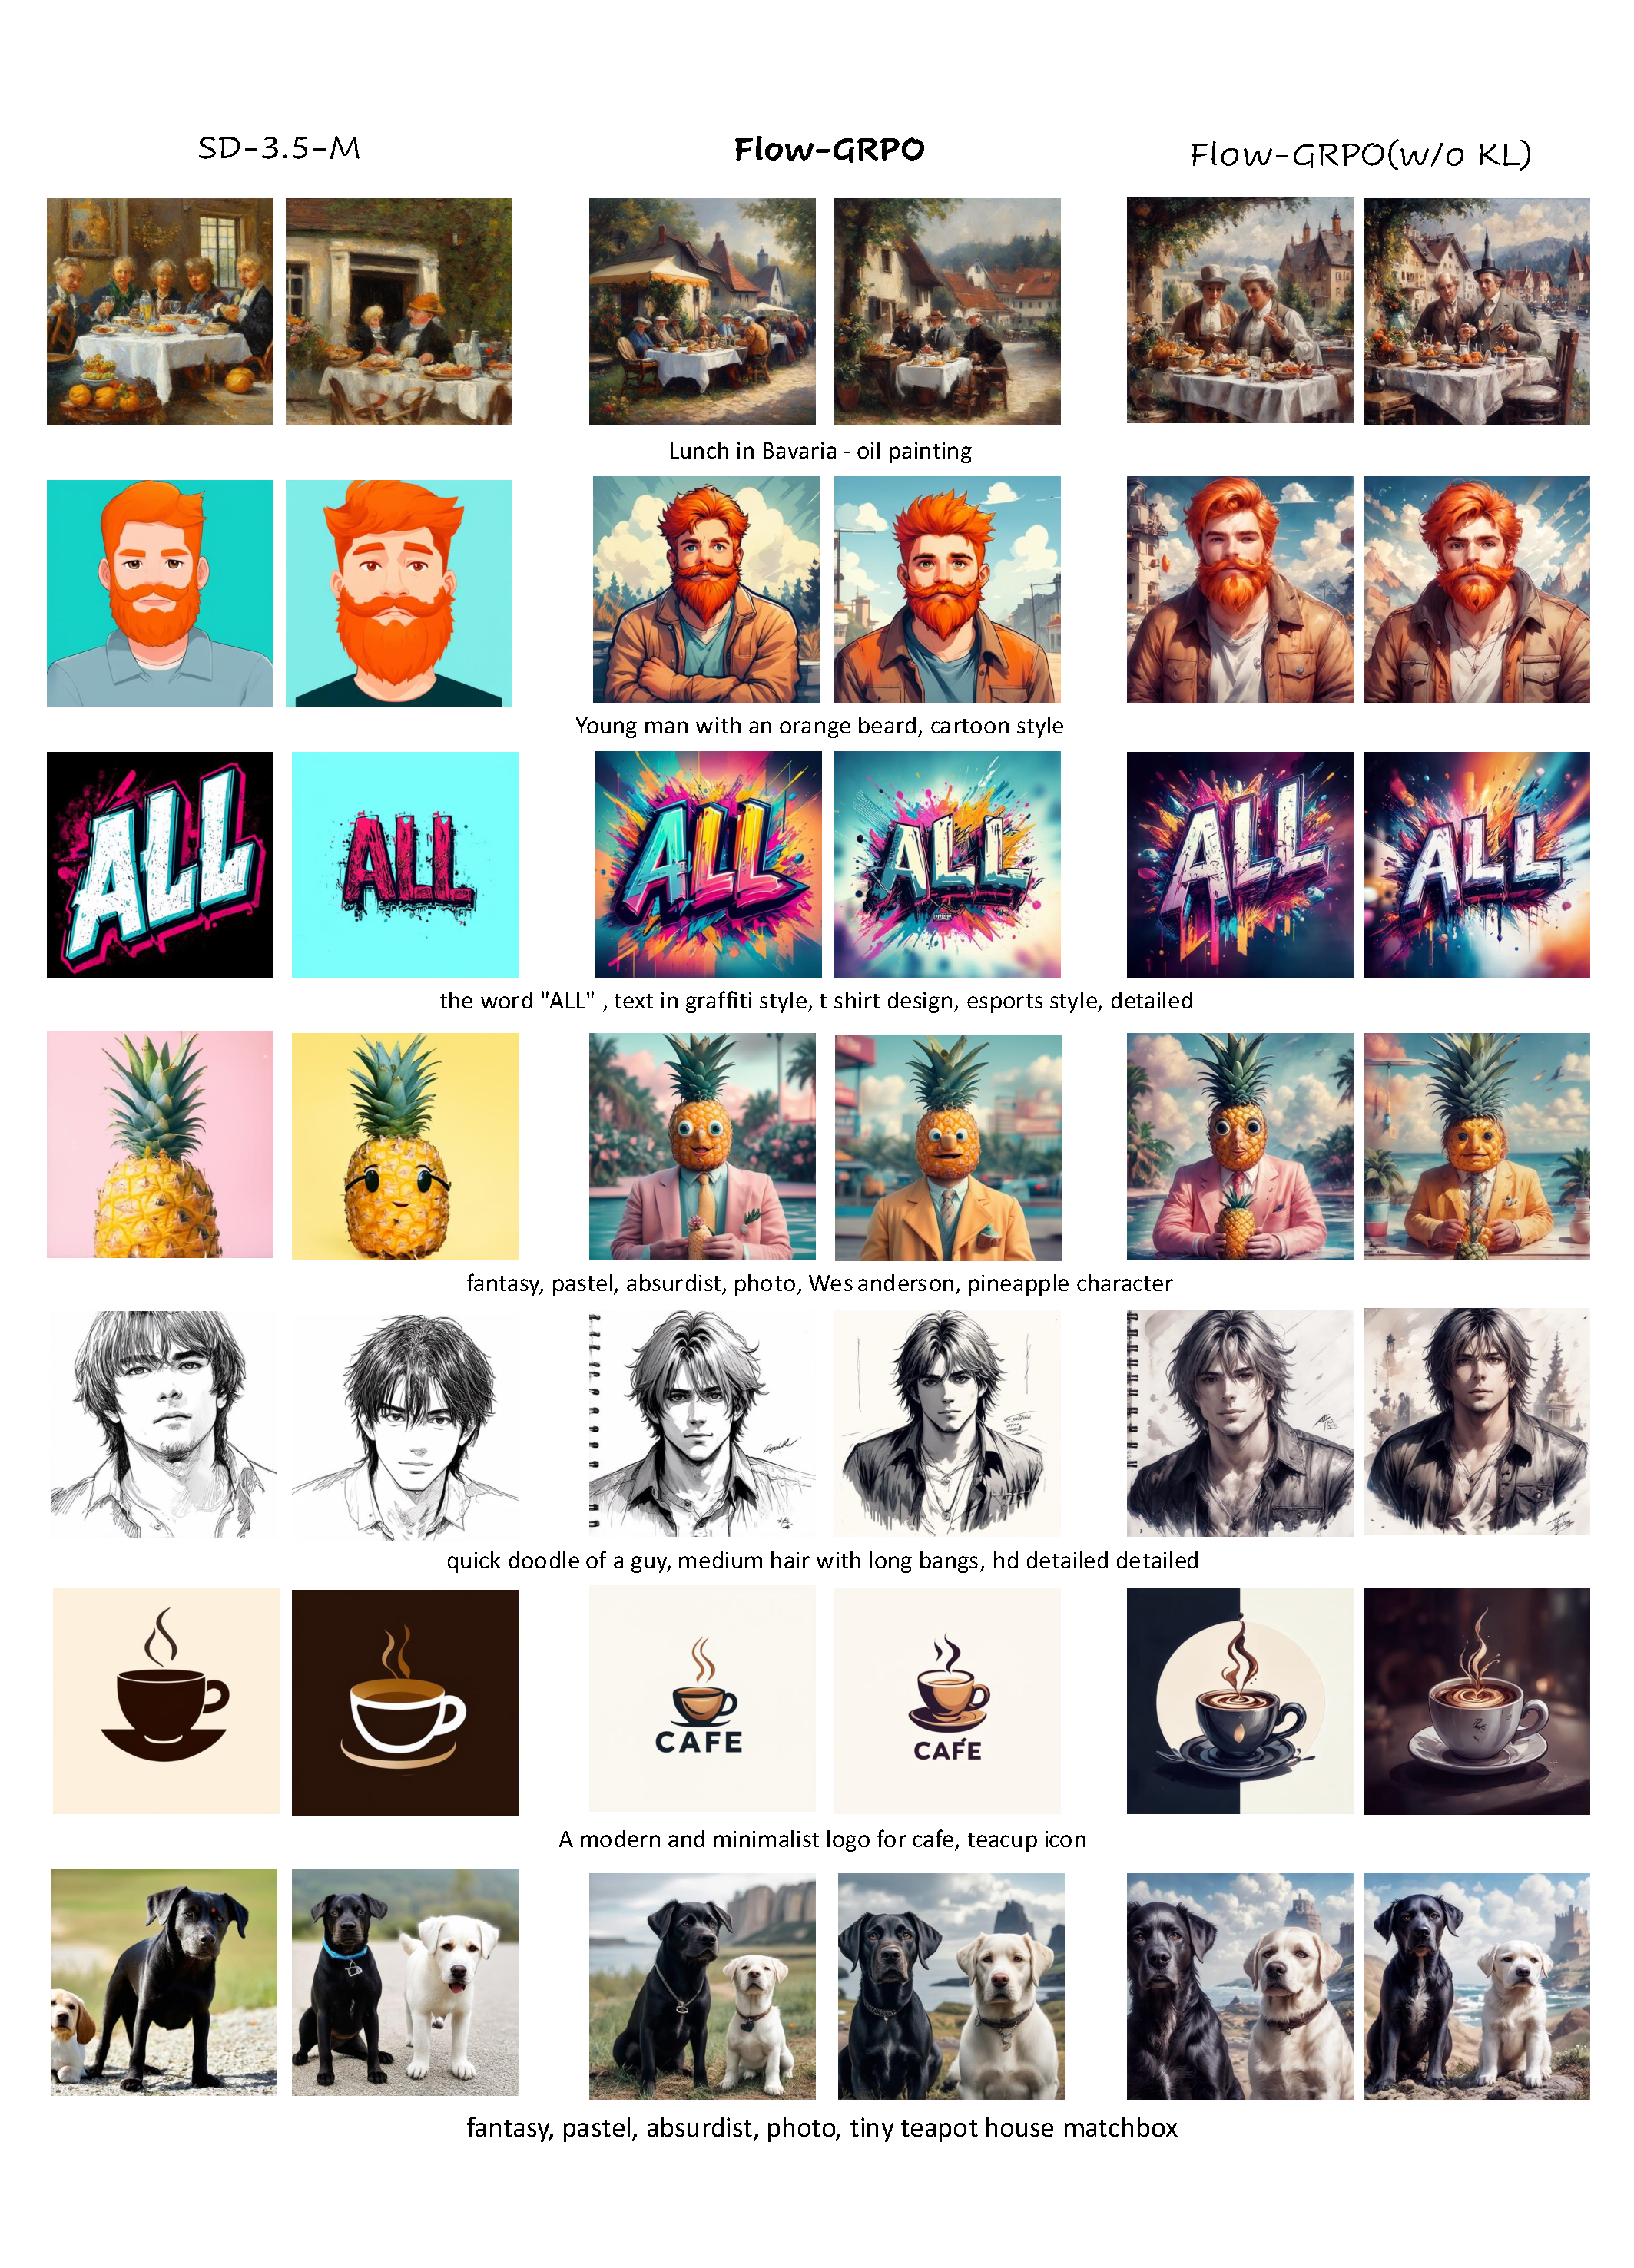
\includegraphics[width=\textwidth]{src/experiments/more_results_pickscore.pdf}
\caption{Additional Qualitative comparison between the SD3.5-M and SD3.5-M + Flow-GRPO trained with \textbf{PickScore} reward.
}
\label{app:fig:add_qualitative_result_pickscore}
\end{figure}

\subsection{Evolution of Evaluation Images During Flow-GRPO Training}

% Here we visualize the generation results of the same evaluation prompts at regular training intervals. All samples are generated with 40-steps ODE schedule. 



To better understand the training dynamics of our proposed Flow-GRPO framework, we visualize the evolution of generated samples corresponding to fixed evaluation prompts at regular intervals during training in Figure~\ref{fig:evolve_qualitative_result_geneval},~\ref{fig:evolve_qualitative_result_ocr} \&~\ref{fig:evolve_qualitative_result_picksore}. For consistency, all visualizations are produced using a 40-step ODE-based sampling schedule. These qualitative results provide a visual representation of how the model progressively improves its generation quality and alignment with task objectives over time.



\begin{figure}[htbp]
\centering
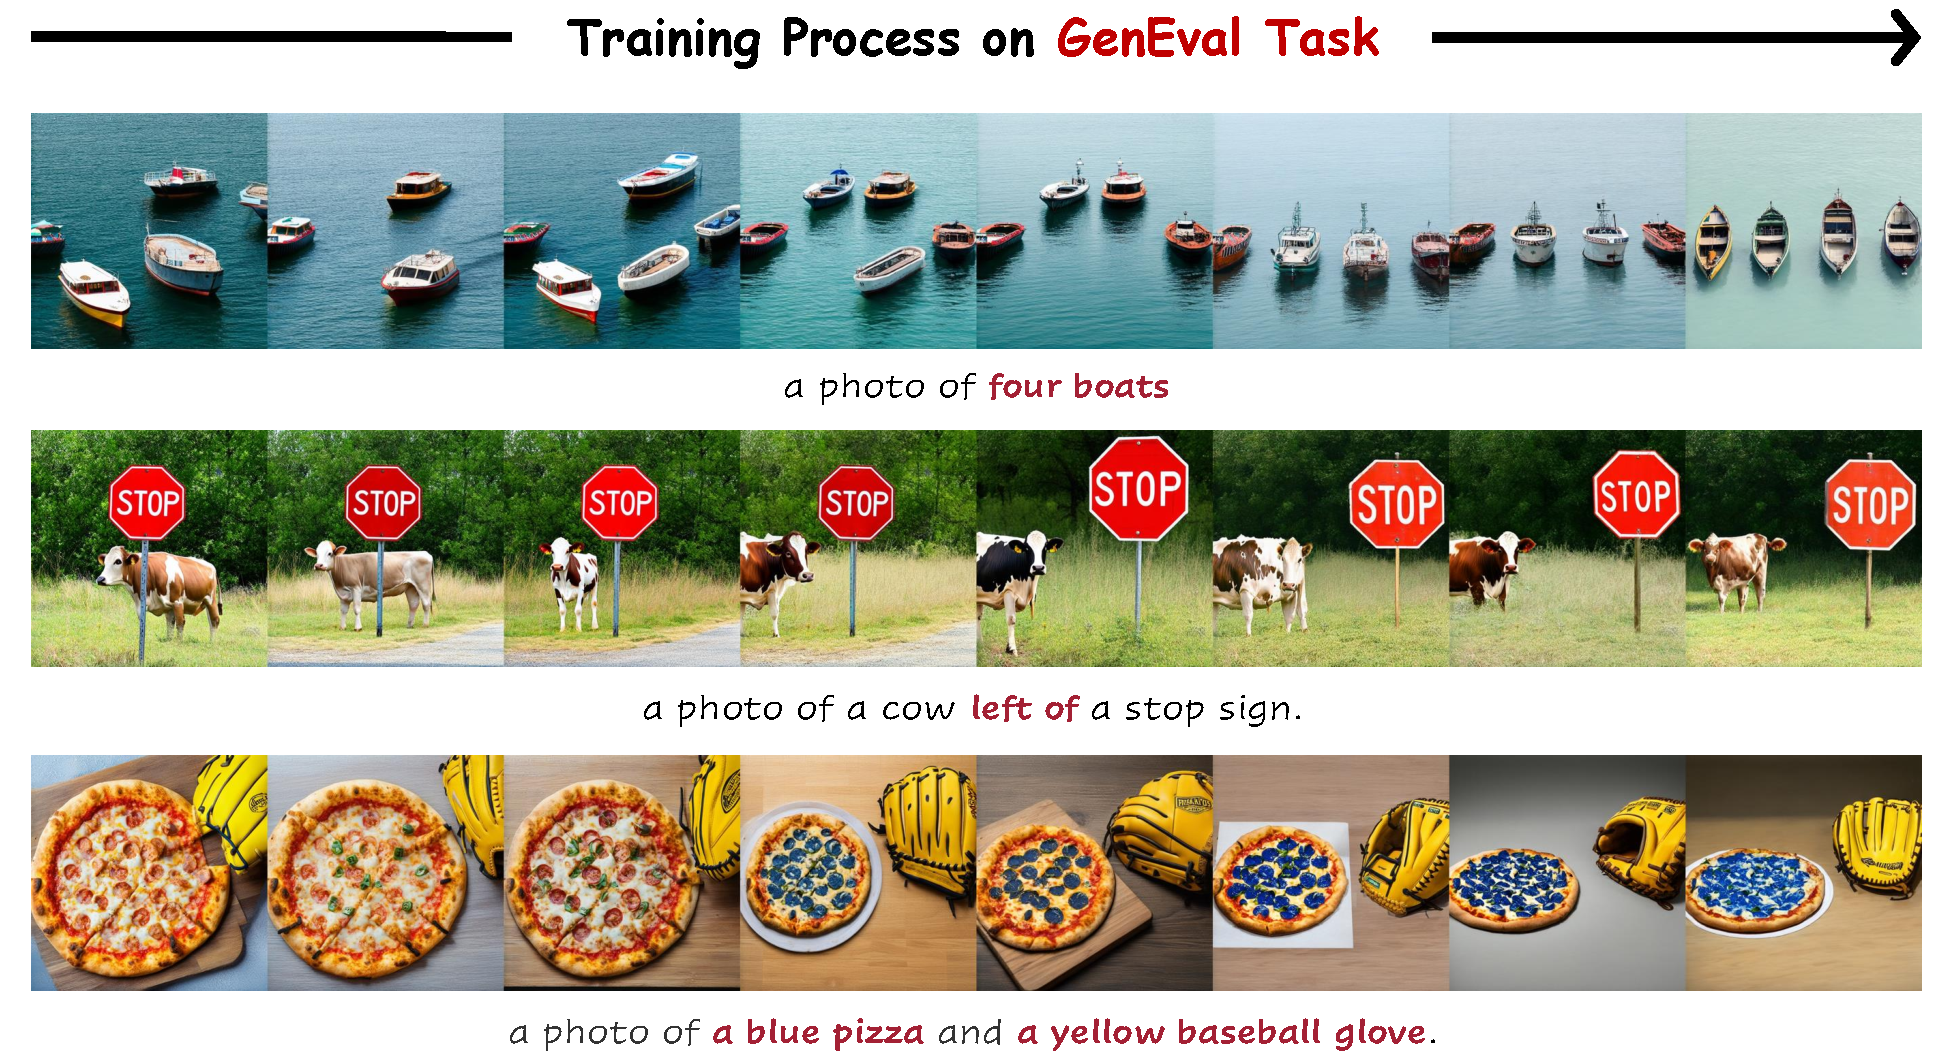
\includegraphics[width=\textwidth]{src/experiments/train_process/train_process_geneval.pdf}
\caption{We visualize the generated samples across successive training iterations during the optimization of SD3.5-Medium on the \textbf{GenEval} task.
}
\label{fig:evolve_qualitative_result_geneval}
\end{figure}

\begin{figure}[htbp]
\centering
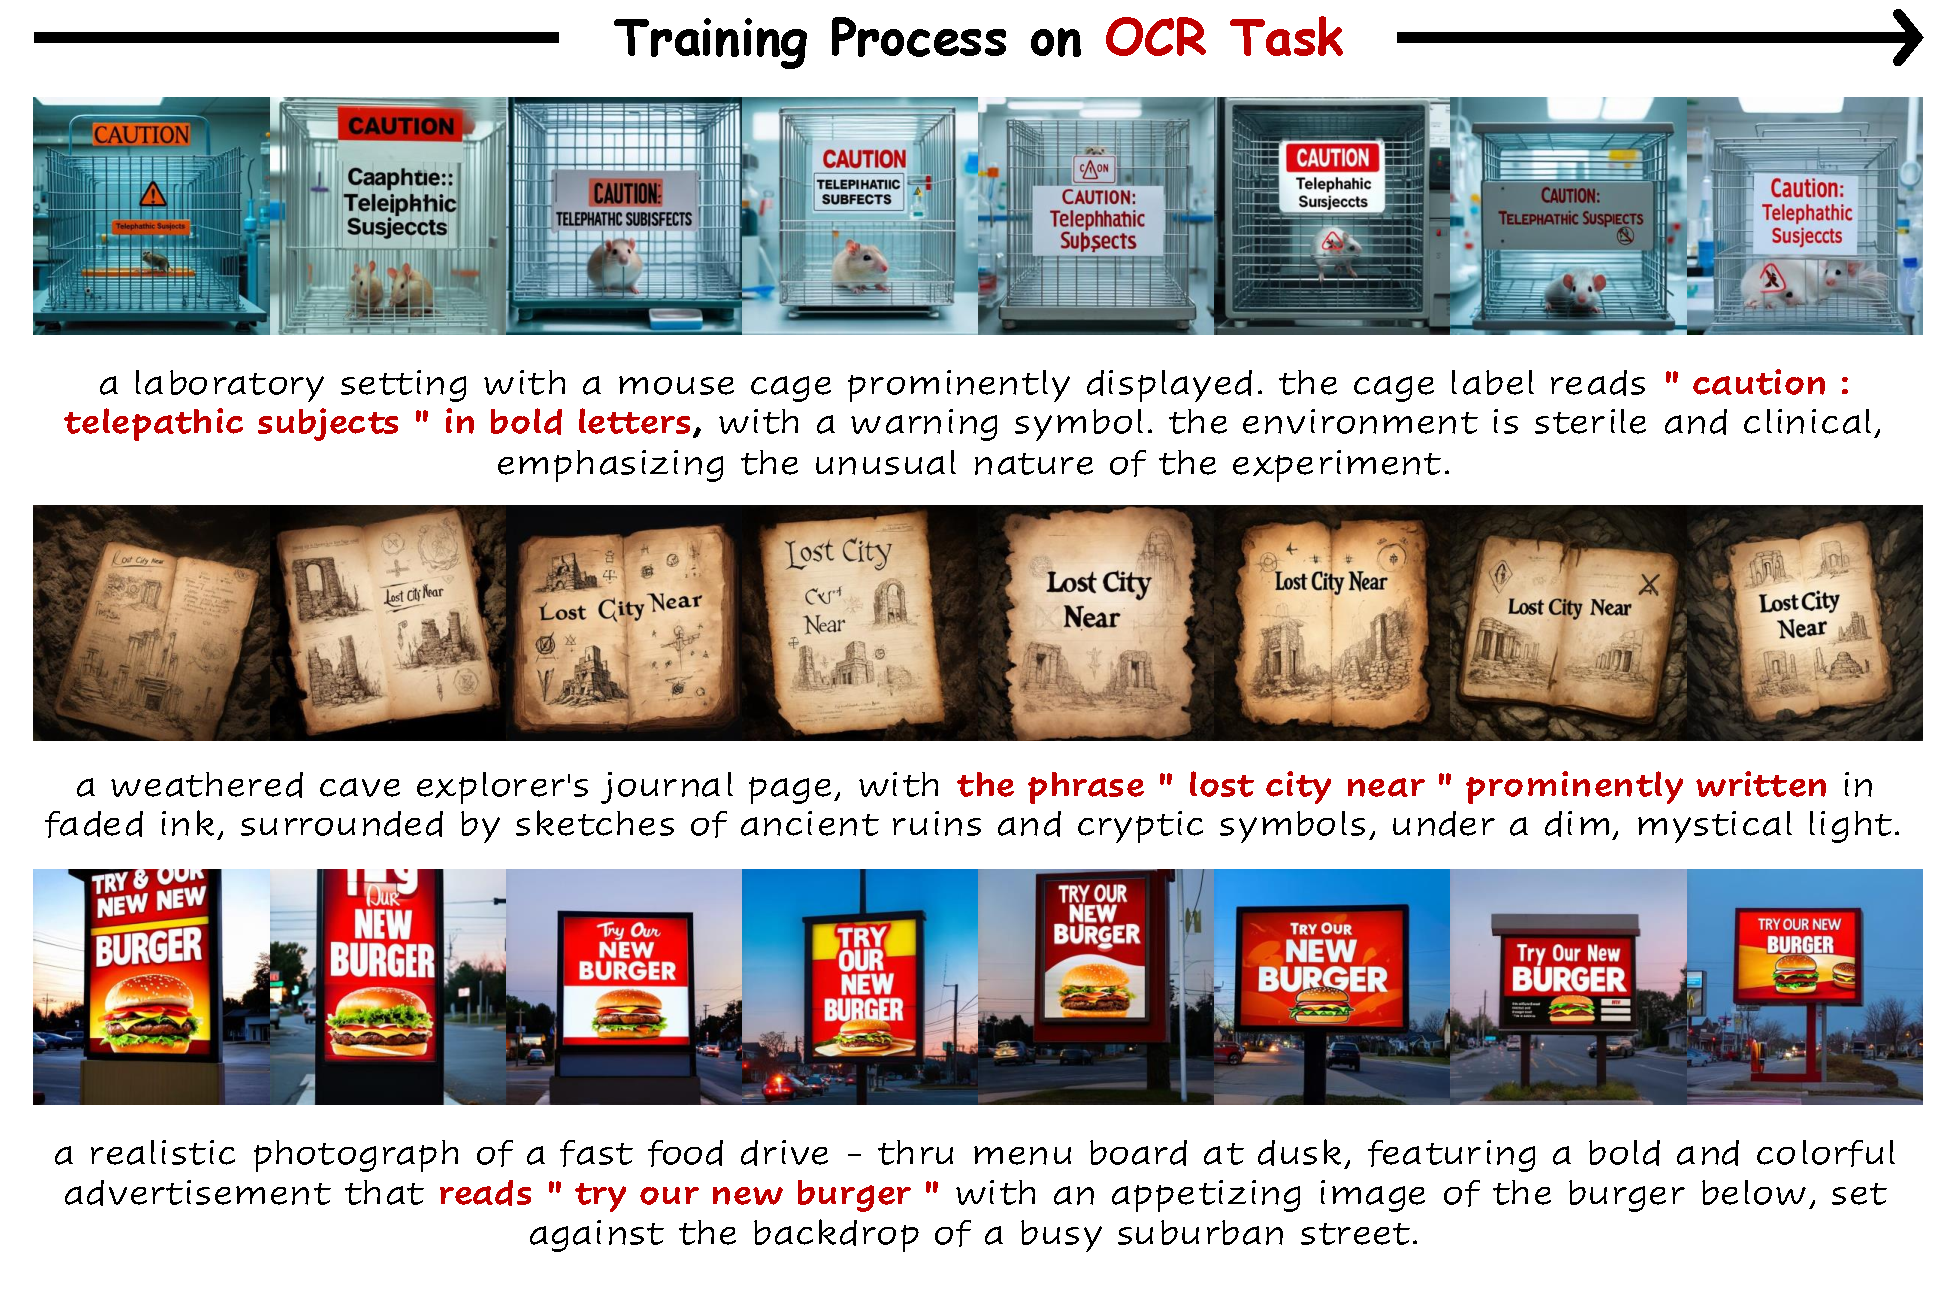
\includegraphics[width=\textwidth]{src/experiments/train_process/train_process_ocr.pdf}
\caption{We visualize the generated samples across successive training iterations during the optimization of SD3.5-Medium on the \textbf{OCR} task.
}
\label{fig:evolve_qualitative_result_ocr}
\end{figure}

\begin{figure}[htbp]
\centering
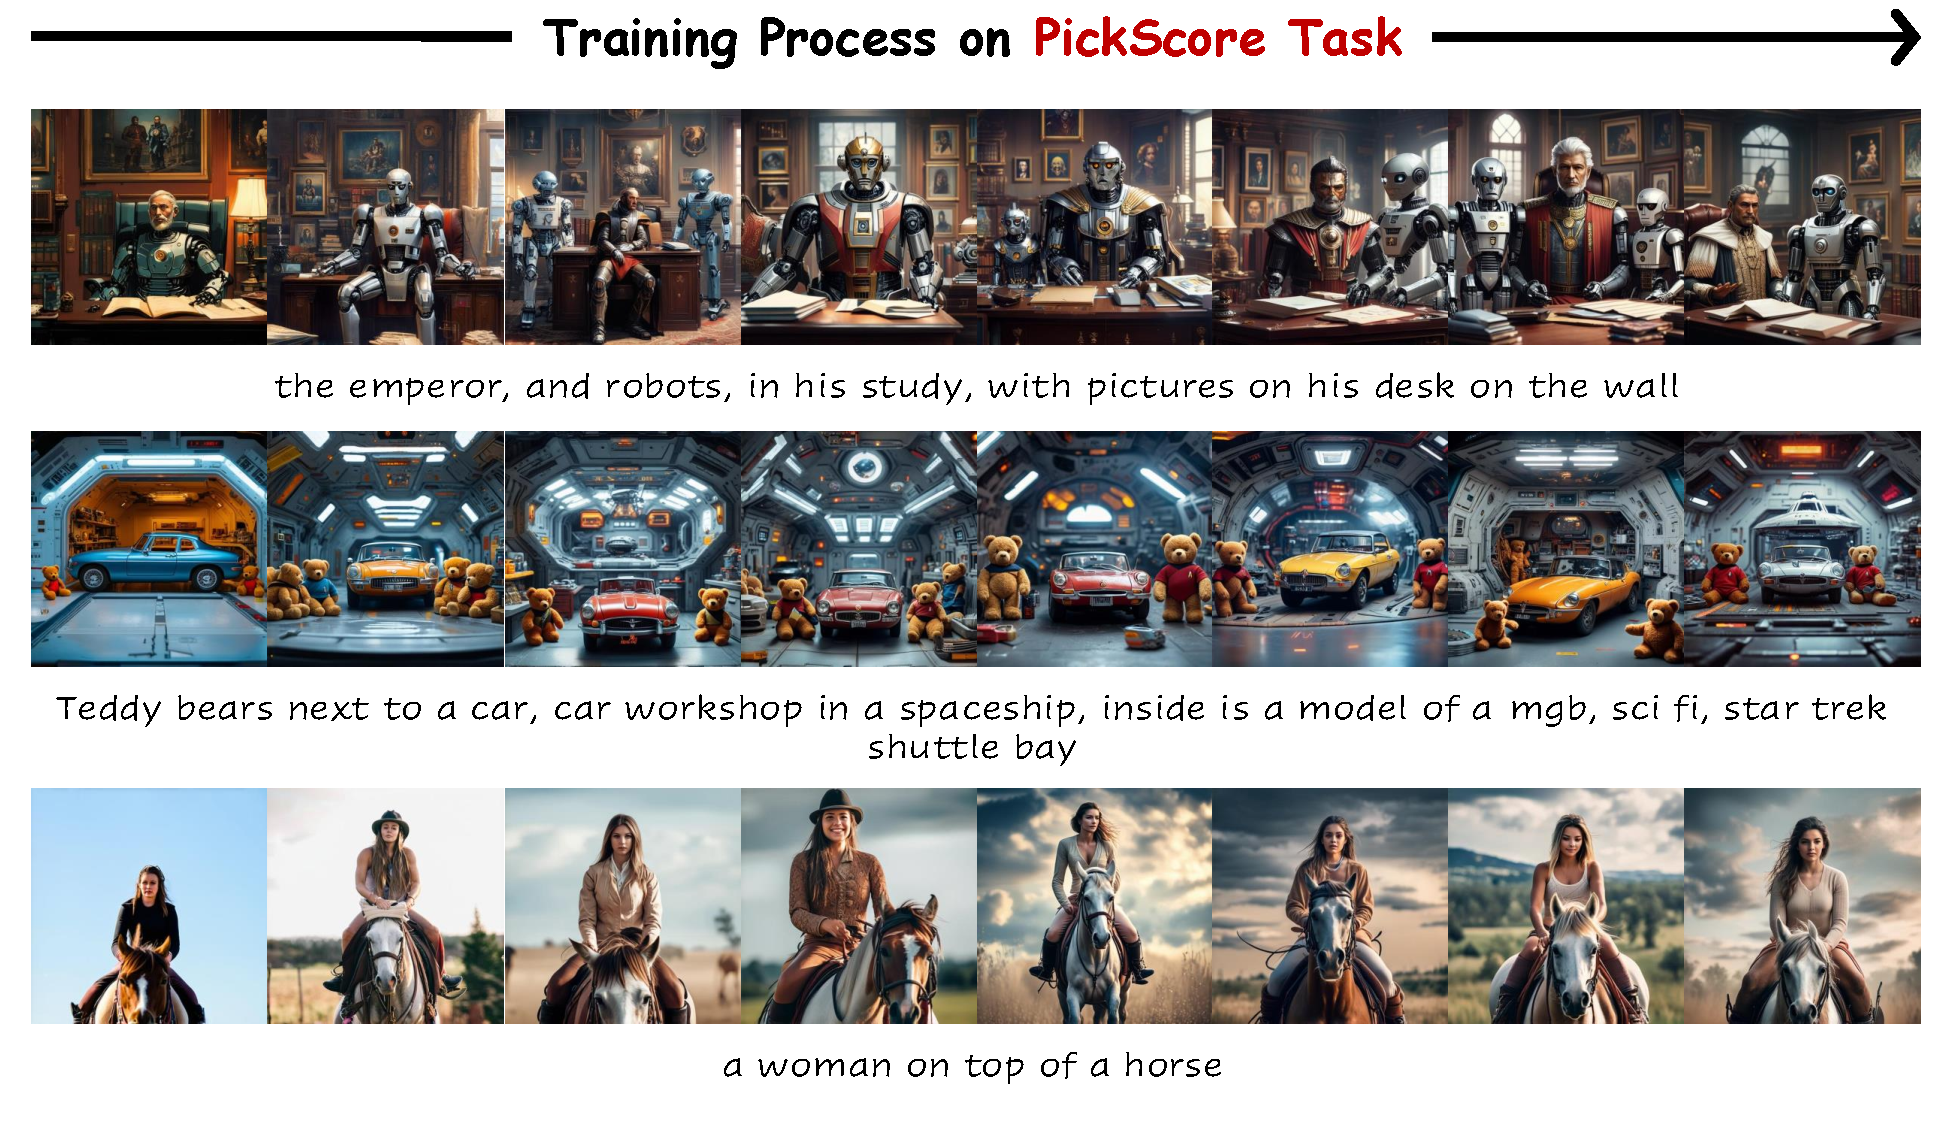
\includegraphics[width=\textwidth]{src/experiments/train_process/train_process_pickscore.pdf}
\caption{We visualize the generated samples across successive training iterations during the optimization of SD3.5-Medium on the \textbf{PickScore} task.
}
\label{fig:evolve_qualitative_result_picksore}
\end{figure}




\section{Training Sample Visualization with Denoising Reduction
}\label{app:sec:denoising_reduction_viz}

In this section, we compare images obtained with SDE sampling at various steps against those produced by ODE sampling, and offer an intuitive view of the denoising reduction strategy.
Figure~\ref{fig:denoising_reduction_viz} presents SD3.5-Medium samples under four inference settings:
(a) ODE sampling with 40 steps;
(b) SDE sampling with 40 steps;
(c) SDE sampling with 10 steps;
(d) SDE sampling with 5 steps.

The 40-step ODE and SDE runs yield visually indistinguishable images, confirming that our SDE sampler preserves quality. 
Shortening the SDE schedule to 10 and 5 steps introduces conspicuous artifacts, like color drift and fine details blur. 
Contrary to expectation that such low-quality samples might hinder optimization. it actually do just the opposite and accelerate optimization. 
Because Flow-GRPO relies on relative preferences, it still extracts a useful reward signal, while the shorter trajectories signifactly cut wall-clock time.
Consequently, Flow-GRPO with denoising reduction strategy converges more quickly on both layout-oriented benchmarks such as GenEval and quality-focused metrics such as PickScore, without sacrificing final performance.


\begin{figure}[htbp]
\centering
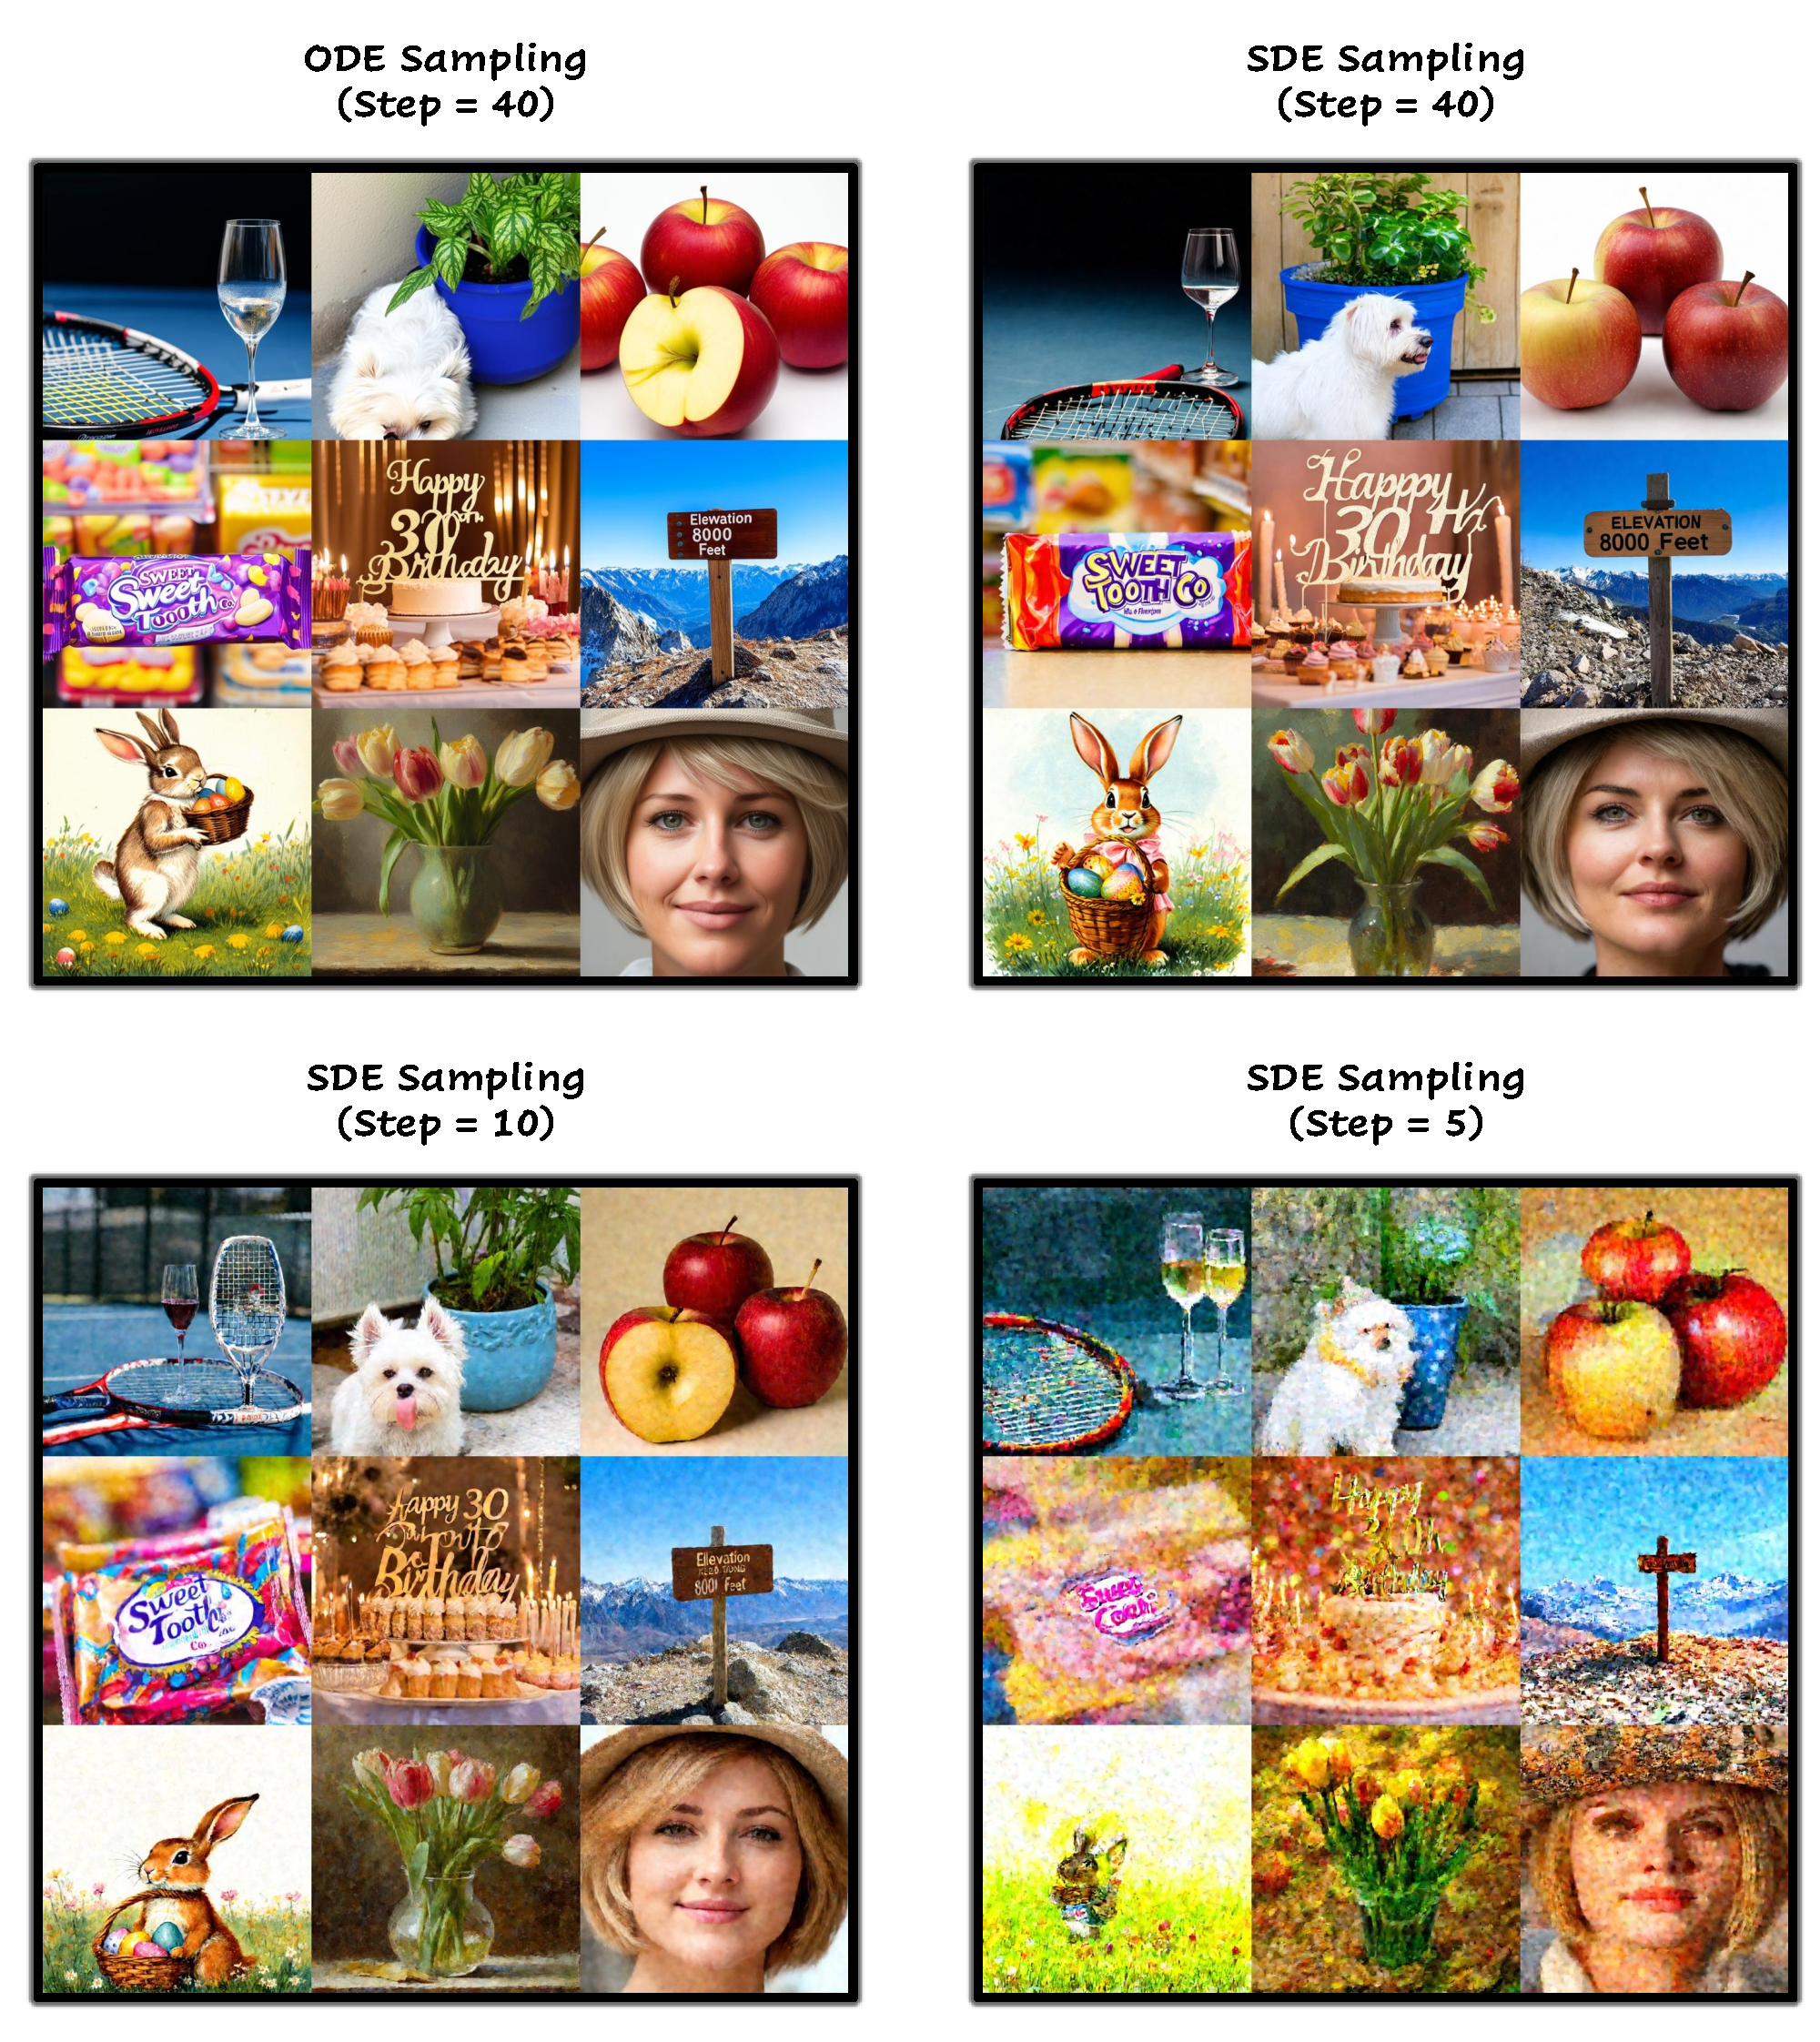
\includegraphics[width=\textwidth]{src/experiments/sampling_viz.pdf}
\caption{Visualization of training samples under difference inference settings.
}
\label{fig:denoising_reduction_viz}
\end{figure}